%%%%%%%%%%%%%%%%%%%%%%%%%%%%%%%%%%%%%%%%%%%%%%%%%%%%%%%%%%%%%%%%%%%
%% This document is part of the set of template files
%% for the uwyo_thesis style. This is your main file that
%% helps compile the entire document; each individual chapter
%% should be a separate file that is brought in using the
%% "\include{}" commands shown below.
%%
%% Step one: rename this file to something specific to you, such as
%% "Smith_thesis.tex" so your eventaul PDF file will end up having the
%% name "Smith_thesis.pdf."  You can also rename any individual chapter
%% files; if you do, be sure to make the appropriate change to the
%% "\include{}" commands below.
%%
%% Important: only *this* file should be compiled by LaTeX.
%% The individual chapter files are *not* standalone files.
%%
%% For interdisciplinary programs such as Neuroscience, see the
%% special section below
%%%%%%%%%%%%%%%%%%%%%%%%%%%%%%%%%%%%%%%%%%%%%%%%%%%%%%%%%%%%%%%%%%%

%%%%%%%%%%%%%%%%%%%%%%%%%%%%%%%%%%%%%%%%%%%%%%
%\documentclass[12pt,oneside,openany]{book}  % single-sided printing
\documentclass[12pt]{book}                  % double-sided printing
%% First line above assumes single-sided printing.
%% For double-sided (duplex) printing use the second line instead.
%% The duplex printing version is best for your final version of the document
%%%%%%%%%%%%%%%%%%%%%%%%%%%%%%%%%%%%%%%%%%%%%%
\usepackage{uwyo_thesis} % the main style file
%%% Many common packages are already loaded by the style file
%%% Add any others below
%\usepackage{??}
\usepackage{graphicx}
\usepackage{latexsym}
\usepackage{array,multirow}
\usepackage{rotating}
\usepackage{tabularx}
\usepackage{setspace}
\usepackage[utf8]{inputenc}

\usepackage{amsmath,amssymb}

\usepackage{booktabs}


%%% Note about your title:
%%% Due to limitations in the UW Banner system, you may want to limit your
%%% thesis/dissertation titles to the following:
%%%  Masters thesis titles:  214 characters including spaces
%%%  Ph.D. dissertation titles: 208 characters including spaces



%%%%%%%%%%%%%%%%%%%%%%%%%%%%%%%%%%%%%%%%%%%%%%%%%%%
%%% set these values for your particular document and
%%% uncomment the lines below as needed
%%%%%%%%%%%%%%%%%%%%%%%%%%%%%%%%%%%%%%%%%%%%%%%%%%%
\mastersthesis % uncomment this if a Masters thesis; comment out if PhD
%\thesisdraft  % uncomment to put time/date/draft stamp in header
%\renewcommand{\thesisauthorLname}{your last name}
%\renewcommand{\thesisauthorFMname}{your first name and middle initial}
%\renewcommand{\thesismonth}{your graduation month}
%\renewcommand{\thesisyear}{your graduation year}
%\renewcommand{\thesisDefenseDate}{the exact day you defend your thesis}
%%% NOTE: you must enter the same title for both \thesistitle and \abstitle below
% Do not use all upper case! That will be done for you where needed.
%\renewcommand{\thesistitle}{your document title}
%\renewcommand{\abstitle}{\ul{your document title}}
% Must be exactly the same as \thesistitle
%\renewcommand{\thesisDeptName}{your academic department or interdisciplnary program}
%\renewcommand{\thesisDeptHead}{name of your academic department head or program chair}
%\renewcommand{\thesisCollegeName}{your college}
%\renewcommand{\thesisDeanName}{name of your college Dean}
%\renewcommand{\thesisDegreeArea}{what your degree is in}
%\renewcommand{\thesisauthorpreviousdegrees}{any of your previous degrees}
%\renewcommand{\lstlistlistingname}{my program listings} % if you want an alternate name for the list
%\renewcommand{\thesisDeptHeadTitle}{Interim Head} % if you're between Dept Heads
%\renewcommand{\thesisDeanTitle}{Interim Dean} % if you're between Deans

%\renewcommand{\thesisdedication}{your dedication} % no length limit, but don't get carried away!

%%%%%%%% Interdisciplinary programs section %%%%%%%%%%%%%%%%%%%
%% You need to define things a bit differently:
%% \renewcommand{\thesisDeptName}{the name of your interdisciplnary program}
%% \renewcommand{\thesisDeptHead}{name of your interdisciplinary program chair}
%% \renewcommand{\thesisDeptHeadTitle}{Program Chair}
%% \renewcommand{\thesisCollegeName}{University of Wyoming}
%% \renewcommand{\thesisDeanName}{name of the UW Provost}
%% \renewcommand{\thesisDeanTitle}{Provost}
%%%%%%%%%%%%%%%%%%%%%%%%%%%%%%%%%%%%%%%%%%%%%%%%%%%%%%%%%%%%%%%


%%% Required: insert your committee member names inside the curly braces
%%% then uncomment the needed lines
% \thesisCommitteeChair{}  % this is your advisor
% \thesisFirstMember{}  % this should be the member *outside* your department
% \thesisSecondMember{}
% \thesisThirdMember{}
% \thesisFourthMember{}
% \thesisFifthMember{}
% \thesisSixthMember{}
% \thesisExternalMember{Carol Danvers}  % a member from another university, not normally used
% only uncomment the line below if you actually have an external member
% \thesisExternalTitle{External Member}  % Not normally used


%%%%%%%%%%%%%%%%%%%%%%%%%%%%%%%%%%%
\begin{document}

% Print initial frontmatter

%%%%%%%%%%%%%%%%%%%%%%%%%%%%%%%%%%%%%%%%%%%%%
%%% Generate the committee page.
%%%  If you want to save a page, you can comment
%%%  this out for early drafts as it isn't needed
%%%  until you're ready for the final version.
%%%
\thesisCommitteePage

%%% the abstract page
\begin{thesisabstract}

When tackling complex combinatorial and AI problems, algorithms can perform very differently on each instance: one might solve it in seconds, while another could fail to resolve within the time limit. This means that algorithms have inherent performance variability across problem instances, resulting in no universally optimal solution. To address this, we can take advantage of the complementary performance of solvers by including them in an algorithm portfolio. This allows us to leverage various portfolio approaches to solve problems more efficiently. 

One of the most studied portfolio approaches is algorithm selection. In this approach, performance models are trained using machine learning algorithms and features extracted from instances. Then, a single algorithm is chosen through the trained model that is estimated to perform well on a specific problem instance. However, selecting a single algorithm might be risky, as machine learning could choose an incorrect solver. Additionally, the advancement of multicore processing technologies provides an opportunity to optimize combinatorial problem solving. One approach to take advantage of multicore systems is to run a large number of solvers in parallel and halt execution as soon as one solver solves the problem. This approach can introduce overhead in shared-resource settings, as the more solvers running in parallel, the more processors will compete for resources. 

This work addresses the limitations of the single-algorithm selection and parallel execution approaches by first including a comprehensive empirical analysis of solvers executed in parallel and direct comparisons of parallel execution versus traditional algorithm selection strategies. This comparison reveals that when there are too many solvers running in parallel, algorithm selection is a better choice. This study also introduces a hybrid model that combines traditional algorithm selection with parallel execution, tailored to instance-specific features, and utilizes uncertainty in algorithm performance predictions. This demonstrated that while algorithm selection generally yields higher efficiency, the proposed hybrid approach significantly improves performance by selecting a per-instance number of algorithms to execute in parallel to make use of parallel processing benefits. In addition, we consider alternative approaches similar to the proposed method and show that the main approach still works better than those alternatives in most cases. These comparisons pave the way for future robust and scalable models in automatic parallel portfolio selection. 

\end{thesisabstract}

\thesistitlepage        % print title page
\thesiscopyrightpage    % print the copyright page
% comment out line below to eliminate the optional dedication page, if you really can't think of anyone!
\thesisdedicationpage   % print the dedication page

% Generate and print the lists
\tableofcontents        % table of contents
\listoffigures          % List of Figures
\listoftables           % List of Tables
% comment out line below if you have no program listings!!!
% \mylistoflistings      % List of program listings


%% acknowledgments section: don't forget to thank your committee
%% members, any funding sources/grants, even your Mom and Dad if you want
\begin{thesisacknowledgments}

I want to express my deepest gratitude to all the incredible people who supported me throughout my PhD journey. Their guidance, encouragement, and support were absolutely essential for my academic success. A special thanks goes to my advisor, Dr. Lars Kotthoff, for his unwavering commitment and countless hours of mentorship. The deep knowledge and patience of Dr. Kotthoff have profoundly influenced my work and my development as a researcher. I am also very grateful to my committee members, Dr. John Hitchcock, Dr. Diksha Shukla, Dr. Suresh Muknahallipatna, and Dr. Mike Borowczak. Their insightful feedback and constructive criticism have been invaluable in improving the quality of my dissertation. I must also acknowledge the support of the National Science Foundation, which funded this research through grant \#1813537, and the School of Computing at the University of Wyoming for their support.

Finally, my heartfelt thanks go to my beloved husband, Ahmad. His support, companionship, and love brightened even the toughest days of this journey. His constant encouragement reminded me that I was never alone.
\end{thesisacknowledgments}


%%%%%%%%%%%%%%%%%%%%%%%%%%%%%%%%%%%%%%%%%%%%%%%%%%%%
%%% Now this is where your various chapters come in
%%%%%%%%%%%%%%%%%%%%%%%%%%%%%%%%%%%%%%%%%%%%%%%%%%%%

%% Abbreviations is an optional entry, placed either at the front or at the end of the document
%% Uncomment the line below if you want abbreviations to be part of the front matter, before Chapter 1
%%%%%%%%%%%%%%%%%%%%%%%%%%%%%%%%%%%%%%%%%%%%%%%%%%%%%%%%%%%%%%%%%%%%%%%%%%%%%
%% This file can be used to generate a list of symbols, abbreviations, etc.
%% as part of the front matter, BEFORE Chapter 1.
%%   For use with theses or dissertations using uwyo_thesis.sty
%%
%%   Version: 1.00
%%   Last modified: 26 August 2019
%%
%%%%%%%%%%%%%%%%%%%%%%%%%%%%%%%%%%%%%%%%%%%%%%%%%%%%%%%%%%%%%%%%%%%%%%%%%%%%%


%%%%%%%%%%%%%%%%%%%%%%%%
\chapter*{Abbreviations, Acronyms, and Symbols}
\label{Abbreviations}  % for you to be able to refer to this appendix in the main text
\addcontentsline{toc}{chapter}{Abbreviations, Acronyms, and Symbols} % make this show up in TOC


% % % % % % % % % % % % % % % % % % % % % % % % % % % % %
{ % begin special environment for abbreviations  -- modify only with great care!

 \setlength{\parindent}{0pt}

%%%%% commands just for this file %%%%%%%%%%%%%%%%%%%%%%%
 \newcommand{\abbrltr}[1]{% command for letter section
   \bigskip
   \framebox{\textbf{#1}}
   \medskip
 }
 \newlength{\abbrwidth}
 \newlength{\abbrdef}
 \setlength{\abbrwidth}{0.9in}  % adjust for longest abbreviation
 \setlength{\abbrdef}{\textwidth}
 \addtolength{\abbrdef}{-\abbrwidth}
 \newcommand{\abbr}[2]{% command for an entry
   \begin{tabular}{p{\abbrwidth}p{\abbrdef}}
     \textbf{#1} & {#2}
   \end{tabular}

 }

%%%%%%%%%%%%%%%%%%%%%%%%%%%%%%%%%%%%%%%%%%%%%%%%%%%%%%%%%
%%%%%%%%%%%%%%%%%%%%%%%%
%% start appendix text %%
%%%%%%%%%%%%%%%%%%%%%%%%

This is a partial list of abbreviations, acronyms, and symbols used in the
text, provided in the hope that it will be helpful to some readers.

\abbrltr{Symbols}

\abbr{$\hat{}$}{Refers to predictions.}

\abbr{$p_{\cap}$}{Threshold for the computed joint probability.}

\abbrltr{Greek Letters}

\abbr{$\mu$}{Mean prediction.}

\abbr{$\sigma$}{Standard deviation of prediction.}

\abbrltr{A}

\abbr{AI}{Artificial Intelligence.}

\abbr{AS}{Algorithm selection.}

\abbr{ASLib}{Algorithm selection library.}

\abbr{ASP}{Answer set programming.}

\abbr{AutoML}{Automated machine learning.}

% \abbrltr{B}

\abbrltr{C}

\abbr{CASH}{Combined algorithm selection and hyperparameter optimization.}

\abbr{CDCL}{Conflict-Driven Clause Learning algorithm.}

\abbr{CNF}{Conjunctive normal form.}

\abbr{COP}{Constraint optimization problem.}

\abbr{CP}{Constraint programming.}

\abbr{CSHS}{Cost-sensitive hierarchical clustering.}

\abbr{CSP}{Constraint satisfaction problem.}

\abbrltr{D}

\abbr{DPLL}{Davis-Putnam-Loveland-Logemann algorithm.}

% \abbrltr{E}

\abbrltr{F}

\abbr{FPGA}{Field-programmable gate array.}

\abbrltr{G}

\abbr{GPU}{Graphical processing unit.}

\abbrltr{H}

\abbr{HPO}{Hyperparameter optimization.}

\abbrltr{I}

\abbr{IP}{Integer programming.}

\abbr{ISA}{Instance-specific ASPEED}

\abbr{ISAC}{Instance-specific algorithm configuration.}

% \abbrltr{J}

\abbrltr{K}

\abbr{KL}{Kullback–Leibler (KL) divergence.}

\abbr{KNN}{K-nearest neighbors.}

\abbrltr{L}

\abbr{LLAMA}{Leveraging learning to automatically manage algorithms.}

\abbrltr{M}

\abbr{MAB}{Multi-armed bandit.}

\abbr{MCP}{Misclassification penalty.}

\abbr{MIP}{Mixed integer programming.}

\abbr{ML}{Machine learning.}

\abbr{MPE}{Most probable explanations}

\abbrltr{N}

\abbr{NP}{Nondeterministic polynomial time.}

\abbr{NFL}{No free lunch theorem.}
% \abbrltr{O}

\abbrltr{P}

\abbr{PAR2}{Penalized average runtime with factor of 2.}

\abbr{PAR10}{Penalized average runtime with factor of 10.}

\abbr{PDDL}{Planning domain definition language.}

\abbr{PPP}{Plain parallel portfolio.}

\abbrltr{Q}

\abbr{QBF}{Quantified boolean formulas.}


\abbrltr{R}

\abbr{RF}{Random forests.}

\abbr{RFJ}{Randomforests model with Jackknife uncertainty method.}

\abbr{RI}{Ranger model with Infinitesimal Jackknife uncertainty method.}

\abbr{RJ}{Ranger model with Jackknife uncertainty method.}

\abbrltr{S}

\abbr{SAT}{Boolean satisfiability problem.}

\abbr{SBS}{Single best solver.}

\abbr{SHAP}{SHapley Additive exPlanations.}

\abbr{SNNAP}{Solver-based nearest
neighbor for algorithm portfolios.}

\abbr{SMT}{Satisfiability modulo theories.}

\abbr{SVR}{Support vector regression.}
\abbrltr{T}

\abbr{TSP}{Traveling salesman problem.}

% \abbrltr{U}

\abbrltr{V}

\abbr{VBS}{Virtual best solver.}

% \abbrltr{W}

% \abbrltr{X}

% \abbrltr{Y}

% \abbrltr{Z}

% % % % % % % % % % % % % % % % % % % % % % % % %
} % end environment for zero \parindent  -- do not remove this curly brace

%\mycleardoublepage

%%%%%%%%%%%%%%%%%%%%%%%%
%%% end appendix text %%%
%%%%%%%%%%%%%%%%%%%%%%%%


 % 

% Bring in the chapter files -- \input is more efficient than \include
% This file is for chapter 1

\chapter{Introduction}

\section{Combinatorial Problems}
Combinatorial problems are computational tasks that arise in various fields, such as computer science and artificial intelligence (AI), and have a wide range of applications. These tasks mainly involve decision-making in arranging, choosing, or assigning elements and primarily deal with finite sets of objects under specific constraints. There are many NP-complete and NP-hard problems that, when focused on discrete optimization and decision-making within a finite set of objects, fall into the category of combinatorial problems.

For example, one well-known problem in this category is the Traveling Salesman Problem (TSP), which is an optimization problem with the objective of finding the shortest path between a finite set of cities, with the constraint of visiting each city at least once before returning to the starting point. TSP is a classic combinatorial problem, and it is categorized as an NP-hard problem, which means that there is no efficient polynomial-time solution for solving the TSP.

\begin{figure}[h]
        \begin{center}
            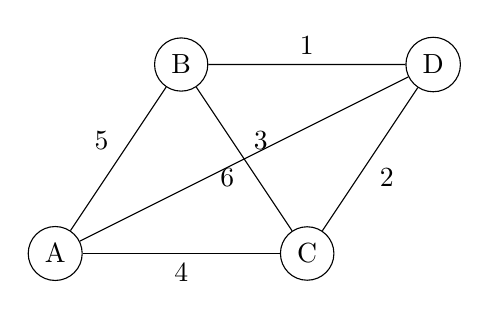
\begin{tikzpicture}[scale=0.8, every node/.style={scale=1}]
                \node[draw, circle] (A) at (0,0) {A};
                \node[draw, circle] (B) at (2,3) {B};
                \node[draw, circle] (C) at (4,0) {C};
                \node[draw, circle] (D) at (6,3) {D};
            
                \draw (A) -- node[above left] {5} (B);
                \draw (B) -- node[above right] {3} (C);
                \draw (C) -- node[below right] {2} (D);
                \draw (D) -- node[below left] {6} (A);
                \draw (A) -- node[below] {4} (C);
                \draw (B) -- node[above] {1} (D);
            \end{tikzpicture}
        \end{center}
        \caption{Traveling Salesman Problem (TSP)}
\end{figure}

Another well-studied example of a combinatorial problem is the Boolean Satisfiability Problem (SAT), which is a fundamental problem in computational theory. Given a propositional formula, the objective is to determine if there is an assignment of truth values to the variables in the formula that makes the formula true \cite{HOOS2005257}. Equation~\ref{eq:int1} shows a simple propositional formula, and the goal here is to find an assignment of Boolean values to each variable that satisfies the entire formula. Many real-world problems can be transformed into SAT problems, including software testing, software verification, bioinformatics, and various optimization problems. SAT is proved to be NP-complete, which means that while a given solution can be verified in polynomial time, finding a solution is challenging, and no polynomial-time algorithm is known to solve all instances of SAT efficiently.

\begin{equation}\label{eq:int1}
        (A \vee B) \wedge (\neg A \vee C) \wedge (B \vee \neg C)
\end{equation}

\section{Overview of Algorithm and Portfolio Selection}
In the domain of combinatorial problems, such as SAT and TSP, the complexity of the problems means that no single algorithm can solve every problem instance optimally. This concept is aligned with the No Free Lunch Theorem, which states that there is no one-size-fits-all algorithm that excels in solving all problems \cite{Karp1972}. 
Research on the development and proposal of innovative algorithms for addressing these problems has a long tradition. These include exact algorithms, approximation algorithms, and heuristics, all of which are widely discussed in the literature \cite{series/faia/336}. 

However, accessibility of a plethora of solvers adds complexity to the problem-solving process, as it makes it difficult to identify the best algorithm for a specific problem. This is because each solver has its unique strengths, weaknesses, and strategies to solve problems. As a result, algorithm performances are often complementary and their performance depends on the characteristics of the instance \cite{Kotthoff2014}, such as the size of the search space and the number of constraints. In other words, within a portfolio of solvers, one solver might solve a particular instance in less than a second, while another could take much longer or even fail within the available time frame. 

In addition, relying solely on the single best solver (SBS) to solve all instances, which often outperforms other algorithms on average, is not always the most effective strategy. Although SBS may be optimal for some, it could be a terrible choice for others. This is illustrated by data from the 2018 SAT Competition (see Figure~\ref{fig:complementarity}), where MapleLCMDistChronoBT was the best performing solver on average for all problem instances. Even the worst-performing solver, Yalsat, outperformed the SBS in certain instances. This shows that the solver considered the worst can, at times, surpass the SBS on specific problem instances. Thus, relying on a single solver to address all problems is inefficient, as it wastes both resources and time. In addition, identifying the best solver for each instance is not feasible without a custom selection process.

\begin{figure*}
    \setlength{\parindent}{0pt}
    \centering
    \includegraphics[width =.9\linewidth]{plots/complementary.png}
\small \caption{Algorithm complementary}
    \label{fig:complementarity}
\end{figure*}

For decades, one of the most prominent ideas in the combinatorial optimization literature has been the concept of designing a portfolio of solvers \cite{GOMES200143,Huberman1997}. This approach does not require extensive knowledge in specific domains, algorithm design, or computational complexity. By treating solvers as black boxes, we can incorporate existing solvers into a portfolio without modifying or designing new ones. This approach allows us to include multiple solvers in the portfolio and take advantage of their complementary strengths, which enables the entire portfolio to excel at solving all problem instances. The actual best solver for each instance, known as the Virtual Best Solver (VBS), which is hard to identify, always exists in the portfolio.

There are different strategies for applying these portfolios to solve problems. Algorithm selection is one portfolio approach that has been studied extensively \cite{Kotthoff2014,10.1162/evco_a_00242}. Algorithm selection techniques are particularly important in solving combinatorial problems, as it is always challenging to choose the best solver for each instance. Selection is not a new problem, and in professional settings or daily life, we often select strategies and things that best fit the situation at hand. In Algorithm selection method, the goal is to identify the most suitable algorithm based on the characteristics of the problem. To address the algorithm selection problem, most approaches focus on employing machine learning algorithms to select suitable solvers \cite{BISCHL201641}. Specifically, by extracting instance features and using a history of algorithm performance data on instances, performance models are trained to predict the best solver. 

Despite the significant success of algorithm selection techniques, there is still room for improvement. A common strategy used to do algorithm selection is choosing a single algorithm to solve a problem instance; however, this can increase the risk of selection, as machine learning models may not always generalize well. This means that they can choose an incorrect algorithm that may perform poorly, leading to suboptimal solutions. To mitigate this risk, several studies have shown that employing a more robust strategy, such as dynamically selecting an ensemble of algorithms based on the characteristics of the problem at hand, can be effective \cite{3s,satzilla}.

Classic subportfolio selection methods focus on choosing a fixed subportfolio for all instances \cite{ppfolio}. However, this approach is suboptimal and inefficient, as it overlooks non-dominating algorithms that perform well on specific instances. In contrast, modern subportfolio approaches emphasize the per instance selection of the solvers \cite{satzilla,3s}. Here, algorithm selection plays a key role, which allows the system to leverage the strengths of multiple algorithms by dynamically adapting the selection to each problem instance's specific characteristics. This adaptability reduces the risk associated with selection and ensures that overlooked algorithms in fixed portfolios are utilized when most effective.

Some subportfolio methods focus on running solvers in parallel, while others use a sequential approach. In sequential execution, a selected solver attempts to solve the instance for a portion of the available time. If the instance remains unsolved, another solver is then employed. This approach can be suboptimal if the initial solver is not the best choice. On the other hand, parallel portfolios run multiple solvers simultaneously, stopping the process as soon as one solver successfully solves the instance. The concept of parallel subportfolios has attracted substantial interest in the literature and has shown great potential. 

Most proposed parallel subportfolio techniques have shown performance improvements primarily through simulations, without executing the algorithms in parallel in real-world scenarios. The few approaches that have collected actual parallel performance data have often focused on a limited number of solvers. Consequently, there is limited understanding of the overhead associated with running solvers in parallel. This gap indicates that, while the concept is promising, more robust real-world evaluations are needed to fully understand its benefits and assess the true scalability of parallel subportfolios.

Additionally, running too many solvers in parallel can introduce overhead on shared memory architectures due to potential contention for shared resources. Although some publications have mentioned this issue, it has not been empirically examined. Others have also overlooked this overhead, proposing parallel methods without accounting for it.

\section{Contributions}

\subsection{Comprehensive Empirical Evaluation of Solvers in Parallel}
The preliminary focus of this dissertation is on extensive empirical evaluation of algorithms in different types of problem, including SAT, Planning, and MaxSAT. This work assesses their performance on varying numbers of cores to provide insights into how solvers behave when running in parallel. By evaluating the solvers in diverse parallel settings, we are able to quantify the computational overhead introduced when running solvers in parallel on shared memory systems, a critical aspect that has been largely ignored in previous research. The results provide an estimate of how beneficial parallelization is when running black-box solvers in parallel, and examine the trade-offs between solver performance and computational overhead. This insight helps us identify the optimal level of parallelization that maximizes efficiency without causing excessive overhead. These evaluations provided a unique dataset, which is a valuable addition to the algorithm selection community.

\subsection{Comparison Between Parallel Execution and Algorithm Selection}
Another important contribution of this dissertation is the direct comparison between the parallel execution of algorithm portfolios and the traditional algorithm selection approach, where a single solver is selected based on the characteristics of the problem instance. Based on the results of our empirical evaluations, this study analyzed the performance of these two methods. The goal was to determine whether running multiple solvers in parallel can offer a competitive or superior alternative to selecting the best predicted solver for each instance.

Our results indicate that algorithm selection outperforms parallel execution in most cases. This is because the overhead associated with running multiple solvers in parallel —especially when there are many parallel runs — can lead to resource contention (competition for CPU, memory, and other resources) and increased coordination costs on multicore architectures, which often offset the benefits of parallelization. This study is the first in the literature to offer a head-to-head comparison between these two strategies. The superiority of algorithm selection, as shown in our results, suggests that a more selective approach can achieve better performance than running a handful of solvers in parallel.

\subsection{Development of a Hybrid Subportfolio Selection Approach}
Another contribution is the development of a hybrid approach that combines algorithm selection with parallel execution of solvers. Traditional algorithm selection methods choose a single solver based on the predicted performance for a given problem instance, but this can result in poor performance if the prediction is inaccurate. In contrast, our hybrid approach dynamically selects a subportfolio of solvers based on instance-specific features and runs them in parallel. Specifically, the uncertainty of the predictions made by the algorithm selector model is used to make more informed decisions. The size and composition of the subportfolio are dynamically adjusted for each problem instance using this uncertainty measurement. This "happy middle" approach balances the strengths of per-instance algorithm selection with the benefits of parallel execution. This method leads to significant performance improvements compared to the existing subportfolio designs in the literature. In addition, the selection and size of the subportfolio are dynamic and tailored to each instance.

\subsection{Fairness and Accuracy of Evaluations}
A unique aspect of this dissertation is its focus on the fairness and precision of evaluations. In shared-memory systems, existing studies often rely on theoretical models or idealized runtime assumptions when running multiple solvers in parallel. This does not reflect the actual performance of the solver in a parallel setting. However, this work uses actual runtime data collected from solver executions in a consistent hardware environment. This work provides a more realistic and fair comparison between the proposed hybrid approach and the baseline methods.

\subsection{Variations of the Hybrid Method}
Lastly, acknowledging the superiority of the hybrid method proposed in this work, we considered variations of the method for comparison. Initially, the performance model used was a regression random forest with Jackknife uncertainty estimation \cite{wager2014confidence}, implemented in the randomForest package in R, based on \cite{randomforest}. Another implementation of the random forest algorithm, known for its speed, is Ranger \cite{ranger}, which offers two methods for uncertainty estimation: Jackknife and infinitesimal Jackknife. This work compares the initial model with two models using Ranger. In addition, the proposed method initially introduced a metric to account for the likelihood of algorithms based on the distribution of predictions. This is replaced with the Kullback–Leibler (KL) divergence method, which quantifies how distinct algorithms are based on the distribution curves. Lastly, while our prediction model was initially trained on sequential data, we compared the results using a model trained on both sequential and parallel data.


\section{Organization of Chapters}

This dissertation is organized into six chapters, each addressed different aspects of the research problem and contributed to the overall development of the proposed approach. The chapters are organized as follows.

The first chapter offers an introduction to the research topic, highlighting the motivation for the study and clearly defining the research objectives. It also introduces the key contributions of the dissertation and outlines the literature gaps that this work addresses.

The second chapter reviews the existing literature related to the research problem, ranging from early studies in this community to recent, more promising work on subportfolio selection and scheduling. It includes a discussion of previous works in the fields of combinatorial problem solving, algorithm selection, parallel solvers, and both sequential and parallel portfolio designs.

Chapter three focuses on the first two key contributions outlined earlier. Provides a detailed presentation of the results from the empirical evaluation that compares the performance of solvers in both sequential and parallel execution modes, covering problem scenarios such as SAT, Planning, and MaxSAT. Furthermore, the results are compared to the traditional single-algorithm selection method.

Chapter four introduces the novel hybrid approach developed in this dissertation, which combines algorithm selection with parallel execution. It expands data collection to cover more problem types and discusses the formulation of dynamic subportfolios. It also provides details on how uncertainty in predicted performance can assist in selecting solvers based on instance-specific features. The effectiveness of this hybrid approach is demonstrated through a comparative analysis with existing methods and baseline models. 

Chapter five provides variations of the proposed approach and compares them with the method introduced in the fourth chapter. Comparisons include different implementations of random forest, replacing the likelihood metric with the KL divergence method, and models trained on sequential and parallel data for a comprehensive analysis.


The final chapter summarizes the key findings and contributions of this dissertation. It also outlines potential directions for future research and acknowledges the limitations of this study, including areas for improvement in algorithm selection techniques and parallel portfolio methods. % chapter 1
\input{uwyo_2} % chapter 2
% This file is for chapter 2

\chapter{Is Algorithm Selection Worth It? \\ Comparing Selecting Single Algorithms and Parallel Execution}

The material of this chapter is based on the following publication: 

H. Kashgarani and L. Kotthoff, “Is algorithm selection worth it? comparing selecting
single algorithms and parallel execution,” in \textit{AAAI Workshop on Meta-Learning and
MetaDL Challenge}, vol. 140 of \textit{Proceedings of Machine Learning Research}, pp. 58–64,
PMLR, 2021.


This chapter provides an empirical evaluation of SAT18-EXP solver performance (from the SAT Competition 2018) when running in parallel with other solvers at different levels of parallelism. Using the collected data, we trained two performance models based on the solver's sequential performance data and instance features. We then performed algorithm selection using these selectors to choose the best-predicted solver for each instance, comparing these results to running multiple solvers in parallel. The findings showed that algorithm selection is superior when many solvers run in parallel. The results in this chapter offer preliminary insights for this dissertation, highlighting the importance of selecting an instance-based subportfolio of solvers since, with fewer solvers, the overhead is minimal. The instance based subportfolio approach will be further developed in Chapter 4 and explored with variations in Chapter 5 and 6. 

\section{Abstract}
   For many practical problems, there is more than one algorithm or approach to solve them. Such algorithms often have complementary performance -- where one fails, another performs well, and vice versa. Per-instance algorithm selection leverages this by employing portfolios of complementary algorithms to solve sets of difficult problems, choosing the most appropriate algorithm for each problem instance. However, this requires complex models to effect this selection and introduces overhead to compute the data needed for those models. On the other hand, even basic hardware is more than capable of running several algorithms in parallel. We investigate the tradeoff between selecting a single algorithm and running multiple in parallel and incurring a slowdown because of contention for shared resources. Our results indicate that algorithm selection is worth it, especially for large portfolios.

\section{Introduction}

The performance of algorithms can vary significantly on different problem
instances and there is no single algorithm that performs well in all cases.
We can take advantage of such performance differences and create
algorithm portfolios to combine the complementary strengths of different
algorithms \cite{GOMES200143}. From this portfolio, we can choose the algorithm with the best performance for each problem instance -- this is known as the algorithm selection problem \cite{Rice1976}. This is usually done by using machine learning methods and features extracted from the instances \cite{Kotthoff2014}. Like all machine learning models, such approaches to algorithm selection make mistakes and in some cases choose an algorithm that does not have optimal performance. We can avoid this by exploiting modern multi-core architectures and simply running all algorithms in the portfolio in parallel, see e.g. \cite{sunnycp2}. While in theory optimal in terms of achieved performance, in practice contention for shared resources such as memory
and caches reduces overall performance.

We present, to the best of our knowledge, the first investigation into the
practical implications of running a large number of algorithms in parallel. We show the trade-off between algorithm selection that chooses a single algorithm and exploiting parallel resources and demonstrate that simply running all algorithms in a portfolio in parallel is not a panacea.

\section{Background}

Algorithm selection and other portfolio-based approaches have been applied in many areas of AI to improve performance. The first paper to introduce portfolios for solving hard AI problem considered a relatively simple parallel approach that executes all algorithms in the portfolio at the same time and stops them all as soon as the solution has been found by one \cite{Huberman1997}. \cite{GOMES200143,Hamadi2009} evaluate this strategy for stochastic algorithms and demonstrate that the variance of the time required to solve a problem decreases as the number of parallel runs increases.

This led to further approaches that take advantage of parallel processing by having several algorithms work independently or in cooperation on a given problem instance. \cite{Yun} construct algorithm portfolios for constraint satisfaction problems that are executed in parallel and show performance improvements for up to 16 processors, and \cite{sunnycp2} propose parallel portfolios with a dynamic schedule for up to 8 cores. Similarly, \cite{10.5555/1661445.1661516} show that by splitting the search space into sub-spaces, constraint solving portfolio approaches can take advantage of as many as 128 processors to achieve performance improvements.

For the Boolean satisfiability problem (SAT), simple static hand-crafted
parallel portfolios have been studied by \cite{roussel2012} and
\cite{wotzlawpfoliouzk} combined with a computed resource allocation for each solver. They employ a fixed selection of SAT solvers with good performance independently in parallel for a given number of cores.
\cite{gagliolo2006dynamic} introduce the dynamic algorithm portfolios that run a portfolio of algorithms with different shares of parallel processors along with an online time allocation learning approach. This includes a lifelong-learning approach in which the priority of algorithms is continually updated based on new runtime information.
\cite{petrik2006learning} also propose a method for enhancing
the performance of deterministic algorithms by running multiple algorithms in parallel for the same problem instance.  \cite{3s,Malitsky2012} propose a more sophisticated approach. They select algorithms through an improved k-nearest-neighbor approach and use both dynamic and static scheduling for multiple algorithms from the portfolio to improve the chance that a particular problem instance will be solved within a time limit.

Similarly, \cite{Marius2015} investigate parallel portfolio selection, and
\cite{aspeed} propose an approach to optimally schedule algorithms from a portfolio using answer set programming, while \cite{Gonard2019} take the simpler approach of running a small portfolio of algorithms in parallel for a short amount of time and using algorithm selection to tackle any problem instances that remain unsolved after that. To the best of our knowledge, all previous research has only simulated parallel execution without measuring the actual performance. We investigate the practical ramifications of running more than one algorithm in parallel.

\section{Experimental Setup}

We run algorithms sequentially and with varying degrees of parallelism. We build and evaluate algorithm selection models for sequential execution to be able to compare selecting a single algorithm to run multiple in parallel. We measure performance in terms of penalized average runtime with factor 10 (PAR10) and misclassification penalty (MCP). The PAR10 score is the observed performance unless an algorithm timed out on a particular instance, when the timeout multiplied by the penalization factor is assumed as the runtime. The misclassification penalty is the difference between the performance of the algorithm that was run and the optimal algorithm on the same instance, i.e. it
is always zero for the optimal algorithm.

We compare to the virtual best solver (VBS), which is the optimal algorithm from the portfolio for each problem instance to solve (cumulative misclassification penalty zero), and the single best solver (SBS), which is the algorithm from the portfolio with the best average performance across the entire set of problem instances to solve. The performance of the overhead-free parallel portfolio corresponds to the VBS.

We consider algorithms and problem instances from SAT, a popular application area for algorithm selection. We selected all 400 instances from the main track of the SAT Competition 2018 \cite{Heule2019} and computed their features using the SATzilla feature computation code \cite{satzilla}. We exclude 19 instances for which we were unable to extract features within two hours of computational time, for a total of 381 problem instances.

Our solvers also come from the main track of the 2018 SAT competition; we consider all 39 submitted solvers for a total of 14,859 algorithm runs. We use the same time limit as in the SAT competition; 5000 CPU seconds for solving a single instance. However, we allowed 128 GB of RAM; more than five times what was allowed in the competition. During the parallel runs, the total amount of memory is shared among all running algorithms. We run the algorithms sequentially, 10 in parallel, 20 in parallel, 30 in parallel, and 32 in parallel to fully saturate a machine with 32 cores.

We leverage the algorithm selection benchmark library ASlib \cite{BISCHL201641} and the LLAMA algorithm selection toolkit \cite{LLAMA} for our algorithm selection experiments. We build regression models that predict the performance of each algorithm in the portfolio individually and select the algorithm with the best-predicted performance, and pairwise regression models that predict the performance difference for each pair of algorithms and select
the algorithm with the aggregated best performance difference. We removed constant-valued (and therefore irrelevant) instance features and imputed missing feature values as the mean over all non-missing values of the feature.

For both regression and pairwise regression approaches, we use random forests as
the base machine learning models.
We tune their hyperparameters following
\cite{BISCHL201641}; we consider values of 10 to 200 for the \texttt{ntree}
hyperparameter and 1 to 30 for \texttt{mtry}. We optimize the hyperparameters
using random search with 250 iterations and perform a nested cross-validation
with 10 external and three internal folds to ensure unbiased performance
measurements. All other hyperparameters were left at their default values.

\begin{table*}[htb]
\centering
\begin{tabular}{l c c }
\toprule
\# parallel runs & \# timeouts & \# out of memory errors\\
\midrule
1 & 6982 (47\%) & 0 (0\%)\\
10 &  10281 (69.19\%) & 6 (0.04\%)\\
20 &  11853 (79.77\%) & 20 (0.13\%)\\
30 &  12590 (84.73\%) & 27 (0.18\%)\\
32 &  12715 (85.57\%) & 5 (0.03\%)\\
\bottomrule
\end{tabular}
\small \caption[Unsuccessful Runs for Each Level of Parallel Execution]{Unsuccessful runs for each level of parallel execution. The numbers in parentheses show the percentage of total runs that the number of unsuccessful runs corresponds to and are rounded to two decimal digits.}
\label{tab:errors}
\end{table*}

\section{Results}

\begin{table*}[htb]
\centering
\smallskip\begin{tabular}{l c c c c c} 
\toprule
metric & \# parallel runs & VBS & SBS & regression & pairwise regression\\
\midrule
PAR10 & 1 & 9256.089
 & 17585.66
 & 13004.31
 & 12588.44

 \\
& 10 & 13062.16
 & 27251.34
 & 19888.25
 & 20410.18

 \\
& 20 & 17099.23
 & 33630.54
 & 25233.38
 & 24970.07

 \\
& 30 & 19970.29
 & 36498.11
 & 28628.15
 & 27317.29

 \\
& 32 & 21674.1
 & 37285.5
 & 29937.23
 & 28888.24

\\ 
\midrule
MCP & 1 & 0 
& 1006.738 
& 441.0526 
& 379.5133
 \\
& 10 & 0 
& 1433.268 
& 684.2932 
& 733.7837
 \\
& 20 & 0 
& 1649.426 
& 811.264 
& 784.1721
 \\
& 30 & 0 
& 1645.936 
& 862.5388 
& 732.7824
 \\
& 32 & 0 
& 1556.284 
& 822.1427 
& 718.0386
\\
\bottomrule
\end{tabular}
\small \caption[PAR10 and MCP Performance Analysis: Comparing Algorithm Selection and Parallel Execution]{Performance in terms of PAR10 score and misclassification penalty for different numbers of algorithms run in parallel. The VBS is the performance of the parallel portfolio; SBS is shown for comparison. The ``regression'' and ``pairwise egression'' columns show the performance of the respective algorithm selection models.}
\label{tab:values}
\end{table*}

\begin{figure*}[htb]
    \setlength{\parindent}{0pt}
    \centering
    \includegraphics[width=0.48\linewidth]{PAR10}\\
    \includegraphics[width=0.48\linewidth]{MCP}
\small \caption[PAR10 and MCP Performance Analysis: Comparing Algorithm Selection and Parallel Execution]{Performance in terms of PAR10 score and misclassification penalty for different numbers of algorithms run in parallel. The VBS is the performance of the parallel portfolio; SBS is shown for comparison. The regression and pairwise regression bars show the performance of the respective algorithm selection models. We omit the plot for VBS performance in terms of MCP score as it is always zero by definition.}
    \label{fig:values}
\end{figure*}

We first evaluate the effect the number of parallel runs has on what fraction of all algorithm runs is successful. Table~\ref{tab:errors} shows the number and percentage of unsuccessful runs at each level of parallelism. With only one algorithm running at a time, 47\% of runs fail with a timeout. This increases as more and more algorithms are run in parallel. Similarly, the number of runs that fail because they run out of memory increases, as more and more runs share the same amount of physical memory. This does not significantly affect the results though, as even in the worst-case much less than 1\% of the total number of runs
is affected. Parallel runs have a much more significant effect on the number of timeouts though -- from 47\% runs that exceeded the available time when only a single algorithm is running at a time, we see an increase to 85.57\% of total runs when 32 algorithms are run in parallel. Altogether, 85.6\% of runs either time out or run out of memory when 32 algorithms are running in parallel; a significant increase over running only a single algorithm.

Table~\ref{tab:values} and Figure~\ref{fig:values} show the performance we
observed for all parallelism levels and approaches we consider. The PAR10 score
for the VBS increases significantly as we increase the number of algorithms run
in parallel; $\approx$41\% from one to 10 parallel runs. Similarly, the score
for the single best solver increases by $\approx$55\% for the same interval. The
PAR10 score is more than twice as high for 32 parallel runs compared to a single
run for both VBS and SBS -- contention for shared resources has a significant
impact on the time it takes to solve a set of instances. A large contributor to
the increase in PAR10 score is the increased number of unsuccessful runs because
of timeouts or memory outs.

We observe a similar decrease in performance as for the VBS and SBS for the algorithm selection approaches as the level of parallelism increases -- in fact, we observe even steeper performance losses in the beginning, with $\approx$53\% performance decrease from one algorithm to 10 for regression models and $\approx$62\% for pairwise regression models in terms of PAR10. However, we observe a performance increase for both approaches (lower MCP scores) when going from 30 algorithms run in parallel to 32, and a performance increase for pairwise regression model when going from 20 algorithms run in parallel to 30. It is unclear what exactly causes this performance increase; it is likely that the machine learning task that underlies the selection process becomes easier as more algorithms lose competitiveness because of timeouts and memory limits.


\begin{figure*}
    \setlength{\parindent}{0pt}
    \centering
    \includegraphics[width =.54\linewidth]{percentage}
    \small 
    \caption[PAR10 Score Increase with More Parallel Runs]{Percentage increase in terms of PAR10 score for running different numbers of algorithms in parallel compared to algorithm selector performance for choosing a single algorithm. For example, an increase of 100\% means that running the algorithms in parallel doubles the PAR10 score over selecting a single algorithm.}
    \label{fig:percentage}
\end{figure*}

Our results show that algorithm selection for choosing a single algorithm to run can beat parallel execution in practice for a large number of solvers. Figure~\ref{fig:percentage} shows that the performance of both the regression and pairwise regression algorithm selection approaches are better than the VBS for any level of parallelism beyond running a single algorithm. Both in terms of PAR10 and MCP, algorithm selection is always better than the single best solver. When using all 32 cores we have available, the VBS becomes more than 66\% worse than the regression algorithm selection approach and more than 72\% worse than
the pairwise regression algorithm selection approach. Even when running only 10 algorithms at the same time (and assuming that we know which 10 of the 39 total algorithms to run to maximize performance), the VBS is more than 0.4\% and 3\% worse than regression and pairwise regression approaches, respectively.

While the overhead-free parallel portfolio promises optimal performance, in theory, we clearly see that in practice this is not the case -- contention for shared resources and physical limits of the machine that is used to run the algorithms has a significant detrimental effect on performance. Even though algorithm selection models are not perfect, they outperform actual parallel portfolios in terms of observed performance even for a relatively small number of algorithms run in parallel.

\section{Conclusions and Future Work}

We investigated the actual observed performance of parallel
portfolios, in contrast to their theoretical performance that is usually used in the literature. We found that running even a relatively small number of
algorithms in parallel on the same machine can have a significant negative
impact on overall performance. Algorithm selection on the other hand chooses only a single algorithm and is able to achieve better overall performance, even though its predictions are not perfect and it does not always choose the algorithm with the best performance for solving a given problem instance.

An obvious avenue for future work is a hybrid approach to what we present here, where instead of a single algorithm several are chosen to run in parallel. Existing literature proposes a multitude of methods for doing so; however, none of these approaches have been evaluated as in the investigation we present here -- by actually running more than one algorithm in parallel and observing the performance rather than simulating this based on the performance observed when only a single algorithm is run at a time. In addition, there is scope for developing new approaches for dynamic resource allocation for algorithm selection.
% Cheat to bring in other references
\nocite{*} % delete or comment this out.
 % chapter 3
% This file is for chapter 3

\chapter{Automatic Parallel Portfolio Selection}

A portion of this chapter has been published as: H. Kashgarani, L. Kotthoff, “Automatic Parallel Portfolio Selection,” in \textit{ECAI 2023}, pp. 1215-1222, IOS Press, 2023.

This chapter introduces a hybrid formulation for dynamic algorithm portfolio selection, which is instance-based and aims to mitigate the risk of selecting a single algorithm or running too many solvers in parallel. The published ECAI paper investigates the results for a random forest regression model trained using the MLR package. Here, in addition to presenting those results, we also expand upon them to explore the transition of regression random forests from the MLR package to its updated version, MLR3, in R.

\section{Abstract}
Algorithms to solve hard combinatorial problems often exhibit complementary performance, i.e.\ where one algorithm fails, another shines. Algorithm portfolios and algorithm selection take advantage of this by running all algorithms in parallel or choosing the best one to run on a problem instance. In this chapter, we show that neither of these approaches gives the best possible performance and propose the happy medium of running a subset of all algorithms in parallel. We propose a method to choose this subset automatically for each problem instance, and demonstrate empirical improvements of up to 23\% in terms of runtime, 83\% in terms of misclassification penalty, and 32\% in terms of penalized averaged runtime on scenarios from the ASlib benchmark library. Unlike all other algorithm selection and scheduling approaches in the literature, our performance measures are based on the actual performance for algorithms running in parallel rather than assuming overhead-free parallelization based on sequential performance. Our approach is easy to apply in practice and does not require to solve hard problems to obtain a schedule, unlike other techniques in the literature, while still delivering superior performance.

\section{Introduction}
For many types of hard combinatorial problems, different algorithms that exhibit complementary performance are available. In these cases, a portfolio of algorithms often achieves better performance than a single one \cite{Huberman1997,GOMES200143}. The algorithms can be run in parallel, or a single one selected for each problem instance to solve. The so-called Algorithm Selection Problem \cite{Rice1976} is often solved using machine learning models which, given characteristics of the problem instance to solve, decide which algorithm should be chosen \cite{Kotthoff2014,10.1162/evco_a_00242}. The machine learning models built for per-instance algorithm selection are not perfect, like most models. In some cases, they lead to choosing an algorithm that does not provide the best overall performance, resulting in wasted resources.

Running all algorithms in parallel avoids this issue, but again wastes resources. Even if the user is only interested in optimizing the elapsed time, i.e.\ it does not matter how many things are run in parallel, results are sub-optimal as parallel executions compete for shared resources such as caches. With more solvers running in parallel, more runs time out, which results in a large overhead. Even for a relatively small number of parallel runs, this overhead becomes prohibitive, resulting in overall performance worse than using imperfect machine learning models to choose a single algorithm \cite{pmlr-v140-kashgarani21a}.

In this chapter, we propose a middle path -- select the most promising subset of algorithms to be run in parallel on a single non-distributed computing machine. This mitigates the impact of both imperfect machine learning models and overhead from parallel runs. We formalize the problem of choosing a subset of algorithms from a portfolio, unifying approaches from the literature. We propose a solution to this problem based on the predictions of algorithm performance models and their uncertainties and compare empirically to other approaches from the literature. We trained three algorithm selection performance models and applied the proposed formulation and could demonstrate improvements of up to 83\% in terms of misclassification penalty, establishing a new state of the art in per-instance algorithm selection with multiple algorithms. We assume that the algorithms to run are not parallelized themselves, i.e.\ each algorithm consumes the same computational resources, and we run on a single machine. We do not consider the case of running algorithms in a distributed setting on multiple machines.

\subsection{Algorithm Selection}
The performance of algorithms designed to solve NP-complete problems, such as Boolean Satisfiability and the Traveling Salesman Problem, can vary significantly depending on the specific problem being addressed. There is no one algorithm that performs optimally in all circumstances. However, we can take advantage of these performance disparities by creating algorithm portfolios that incorporate the complementing strengths of several algorithms \cite{GOMES200143,Huberman1997}. 

The algorithm portfolios proposed in \cite{GOMES200143,Huberman1997} run multiple algorithms in parallel, however, they do not measure the actual execution time when running in parallel but simulate parallel execution based on sequential performance. \cite{pmlr-v140-kashgarani21a} found that the performance of the portfolio can deteriorate substantially when algorithms are executed in parallel, in particular for more than 10 algorithms. \cite{LINDAUER2017272} has also determined that running various configurations of an algorithm in parallel can introduce overhead, and this factor should be considered when designing portfolios. Alternatively, we can choose a subset of the best algorithms from the portfolio for a given problem instance to avoid the overhead of running a large number of solvers in parallel. In the case where we choose only a single algorithm, this is known as the algorithm selection problem~\cite{Rice1976}. Typically, this is accomplished through the use of machine learning techniques and features derived from the instances~\cite{Kotthoff2014,10.1162/evco_a_00242} and algorithms~\cite{pmlr-v188-pulatov22a}. However, choosing only a single algorithm to run often achieves suboptimal performance because of incorrect choices. This can be addressed through better algorithm selection models; in this chapter, we explore the alternative of choosing more than one algorithm to run in parallel on a single node.

Algorithm selection has been applied successfully in many problem domains. Some of the most prominent systems are SATzilla, Hydra, and Autofolio ~\cite{satzilla,lindauer2015autofolio,10.5555/2898607.2898641}. While these systems focus on SAT, algorithm selection also has been used in the constraint programming and mixed integer programming domains, where it has been shown to achieve good performance \cite{cphydra,XuEtAl11}. AutoFolio has been applied in additional areas, e.g.\ ASP, MAXSAT, and QBF. \cite{10.1162/evco_a_00215} apply algorithm selection for the TSP, and ME-ASP \cite{maratea2014multi} apply algorithm selection for answer set programming to create a multi-engine solver. Algorithm selection has also been used to choose between evolutionary algorithms \cite{HU201268, yuen2019selecting, Maturana2012, 9ae8443ad82b4056bccf7102c0056152}.
The ASlib benchmarking library~\cite{BISCHL201641} collects benchmarks from many different problem domains and is the de facto standard library for evaluating algorithm selection approaches.

\par{\textbf{Notation.}}
We follow~\cite{pmlr-v79-lindauer17a} in the notation we use in this chapter.
Given a portfolio of algorithms (solvers) $S$, a set of instances $I$, and a performance metric \begin{math} m: S \times I \to \mathbb {R^+} \end{math}, we aim to find a mapping \begin{math} s: I \to S \end{math} from instances $I$ to algorithms $S$ such that the performance across all instances is optimized. This performance metric can be for example the time needed to solve the instance and we assume w.l.o.g.\ that the performance metric should be minimized. In practice, we estimate the value of the performance metric based on the predictions of machine learning models for new problem instances; we denote this estimate $\hat{m}$. We want to select the solver with the best-predicted performance for each instance:

\begin{equation}\label{eq:1}
    min \frac{1}{|I|} \sum\limits_{i\in I} \hat{m}(s(i),i)
\end{equation}


\subsection{Portfolio Scheduling}
Different approaches have been proposed for sub-portfolio selection. Some approaches choose a number of suitable solvers for sequential execution and assign  time slices that sum to the total available time to each algorithm. Others have implemented parallel execution of the selected solvers, while a few have combined these two methods, utilizing parallelization across computing processors and splitting the available time of each processor across different algorithms. 

\subsubsection{Time slice allocation on single processor}

Typically, sub-portfolio selection strategies are built for sequential solver runs, e.g.\ Sunny~\cite{sunny} creates a sub-portfolio of solvers using k-nearest neighbor (kNN) models and builds a sequential schedule for the selected solvers by allocating time slices based on the predicted performance. CPHydra~\cite{cphydra} also employs case-based reasoning and allocates time slices for the selected CSP solvers to run sequentially. 3S~\cite{3s} dynamically selects and sequentially schedules solvers for a given SAT instance using integer programming. ASPEED~\cite{aspeed} creates static sequential schedules through answer set programming that optimizes a static sequential time budget allocation for solvers. Depending on the number of algorithms, solving the scheduling problem can take substantial time. Building on the methodologies of 3S~\cite{3s} and ASPEED~\cite{aspeed}, ISA (Instance-Specific ASPEED)~\cite{flexfolio} uses kNN to identify the closest training problem instances to a given problem instance to solve. It then employs ASPEED to determine a schedule that minimizes the number of timeouts across these instances. \cite{flexfolio} also introduced TSunny which is a modified version of Sunny that limits the number of solvers to run, thus increasing the chance of success by allocating larger time slices to each algorithm.

\subsubsection{Time slice allocation on multiple processors}

Other portfolio techniques have focused on scheduling solvers to run in parallel and allocating time slots on different processors. P3S~\cite{p3s} is a parallel version of 3S and uses the kNN algorithm for selecting solvers and scheduling them using integer programming with a specific runtime allocation strategy, where it runs a static set of solvers for the first 10\% of the available runtime and solvers selected for the instance for the remaining 90\%. ASPEED~\cite{aspeed} can also define a fixed schedule for running solvers on multiple processors, which is chosen based on the average solver performance across a set of instances. Flexfolio \cite{flexfolio} incorporates a reimplementation of the P3S approach utilizing the same 10-90 strategy. However, rather than employing integer programming to address the scheduling problem, Flexfolio makes use of ASPEED and solves it through answer set programming. Sunny-cp~\cite{sunnycp2} can simultaneously execute multiple CSP and COP solvers. First, a portion of the total available time is allocated to a pre-solving phase that follows a fixed schedule. The remaining time is then distributed amongst the other selected solvers dynamically, based on the predictions of kNN performance models. As there are often more solvers than processors, all processors except one are assigned to the corresponding number of top-ranked solvers, while the time on the final processors is split among the remaining solvers.

\subsubsection{Running algorithms in parallel}

One of the first parallel SAT solvers is ppfolio~\cite{ppfolio}. It selects solver portfolios to solve sets of problem instances optimally, but does this only for entire sets of instances, not on a per-instance basis as we do here.
The success of ppfolio has inspired many other researchers to create sub-portfolios of solvers to run in parallel. For example, \cite{Marius2015} extended existing algorithm selectors like 3S, SATzilla, and ME-ASP to greedily choose the top $n$ solvers to run in parallel by producing a ranking of candidate algorithms; however, the number of solvers has to be specified by the user and the actual runtime of parallel runs is not considered -- the same runtime as for sequential execution is assumed.
Running algorithms in parallel on the same machine is slower than running sequentially in practice due to the overhead incurred because of shared caches and shared memory. This has been shown in experiments~\cite{pmlr-v140-kashgarani21a}, simulations~\cite{Yun,jtom1286288}, and analyses~\cite{biere} for the parallel executions of solvers -- in practice, ignoring the overhead that parallel execution introduces reduces overall performance.

\medskip

In this chapter, we consider the problem of selecting the optimal subset of algorithms to run in parallel on a single machine. This is computationally much easier to solve on a per-instance basis than more complex scheduling approaches, e.g.\ the ones used by ASPEED and 3S, which means that our method is easier to deploy and introduces less overhead. As long as the best solver is part of the selected portfolio, we will achieve optimal performance or close to it, whereas approaches that allocate time slices may choose the best solver, but fail to achieve optimal performance if too little time is allocated to it. We leverage more information from algorithm selection models than most approaches in the literature, in particular the uncertainty of performance prediction. This allows us to trade off the number of algorithms to choose with the chance of success in a principled way. Our approach is designed to optimize the usage of parallel computational resources when solving combinatorial problems while taking into account the overhead that arises from parallel runs. To the best of our knowledge, there are no other approaches that solve parallel algorithm selection this way.

\section{Parallel Portfolio Selection}

We aim to choose a sub-portfolio of solvers \begin{math} P_i \subseteq S \end{math} for a given instance $i \in I$ that includes the algorithms with the best performance on $i$ (\begin{math} A \in S \end{math} and \begin{math} A \in P_i \end{math}) to run in parallel, based on the predicted performance of each solver. Given the predicted performance metric $\hat{m}$, we can define a total order of the algorithms in the portfolio $S$ for a given instance $i$. This total order is induced by the ranking of the algorithms based on their predicted performance for instance $i$. Formally, the total order can be defined as:
\begin{equation}\label{eq:3}
A < B \quad \text{if} \quad \hat{m}(A,i) < \hat{m}(B,i); A,B \in S
\end{equation}

Given the total order, the rank of each algorithm $A$ on each instance $i$ can be defined as the number of algorithms that are predicted to be strictly better than $A$ for the instance and denoted $r_{A,i}$. Ties are broken arbitrarily. A portfolio of a specified size $n$ is then defined as the top $n$ algorithms according to rank for that particular instance. The portfolio of size $n$ for instance $i$ can be expressed mathematically as:
\begin{equation}\label{eq:4}
P_i = \{A \in S \: | \: r_{A,i} \leq n\}
\end{equation}

In a slight abuse of notation, we will denote the rank of an algorithm as a subscript, i.e.\ $r_{A,i}$ is the rank of algorithm $A$ on instance $i$ and $A_{1,i}$ is the algorithm of rank $1$ (the best performing algorithm) on instance $i$.

This allows to choose a subset of algorithms with the best predicted performance for a given instance, which can then be executed in parallel. However, determining the portfolio size $n$ for a given problem instance is the key challenge for parallel portfolios. As discussed above, choosing only a single algorithm or all algorithms is unlikely to give optimal performance in practice. The larger the number of algorithms we include, the larger the chance that the best algorithm is in the chosen portfolio, but also the larger the overhead from running many algorithms in parallel. 

Here, we want to include the algorithms that, according to their predicted performance on a new problem instance, have the highest chances of achieving optimal performance, while also taking into account the computational overhead of running multiple solvers in parallel. We leverage the uncertainty of the predictions of the performance models to gauge the likelihood that a given algorithm would be competitive. To the best of our knowledge, there are no algorithm selection approaches that do this.

Instead of considering only a point prediction, we consider the predicted distribution of performance metric values, characterized by its mean and standard deviation. Formally, we denote the standard deviation of the prediction \begin{math}\hat{m}(A, i)\end{math} as \begin{math}\sigma_{A, i}\end{math} for each solver $A$ and instance $i$.
We assume that the predictions of our performance models follow a normal distribution, i.e.\ the predicted value is the mean of that distribution and allows to characterize it completely together with the standard deviation. We assess the likelihood of two algorithms performing equally well by computing the overlap between their distributions. If two algorithms are predicted to perform very similarly, then the overlap between the distributions will be very large.

We are in particular interested in the predicted performance distribution of the best-predicted algorithm $A_{1,i}$ (no algorithms are predicted to perform better than it), and how the predictions for the other algorithms compare to it.
Formally, for the best predicted solver $A_{1,i}$ on instance $i$ the distribution of predictions is \begin{math} \hat{m}(A_{1,i}, i) \sim \hat{M}(\mu_{A_{1,i},i}, \sigma^2_{A_{1,i},i}) \end{math} with probability density function \begin{math} f_{A_{1,i},i}\end{math} and cumulative distribution function \begin{math} F_{A_{1,i},i}\end{math}. The performance distributions for other algorithms are defined similarly.

For the distributions of the predicted performance of two algorithms $A_x$ and $A_y$ on instance $i$, the point of intersection $c$ can be computed as \begin{math} f_{A_x,i}(c) =  f_{A_y,i}(c) \end{math}. That is, the predicted probability of achieving this particular performance is equal for both distributions (illustrated in Figure~\ref{fig:overlappingarea}).
For \begin{math}
    \mu_{A_x,i} < \mu_{A_y,i}
\end{math}, $c$ is defined as (we omit the index $i$ for the sake of brevity here):

\begin{equation}\label{eq:5}
\resizebox{\columnwidth}{!}{$c = \frac{\mu _{A_y} \sigma _{A_x}^2-\sigma _{A_y} \left(\mu _{A_x} \sigma _{A_y}+\sigma _{A_x} \sqrt{\left(\mu _{A_x}-\mu _{A_y}\right){}^2+2 \left(\sigma _{A_x}^2-\sigma _{A_y}^2\right) \log \left(\frac{\sigma _{A_x}}{\sigma _{A_y}}\right)}\right)}{\sigma _{A_x}^2-\sigma _{A_y}^2}$}
\end{equation}

Given $c$, the overlap between the distributions is defined as the joint probability of $A_x$ performing worse than $c$ and $A_y$ performing better than $c$:

\begin{equation}\label{eq:6}
    p(\hat{m}({A_{x,i}}, i) \geq c) \cdot p(\hat{m}({A_{y,i}}, i) \leq c) = 1 - F_{A_{x,i},i}(c) +  F_{A_{y,i},i}(c)
\end{equation}

We define $p_{\cap} \in [0,1]$ as a threshold for the computed joint probability to include a given algorithm:

\begin{equation}\label{eq:7}
 P_i = \{A \:| \: \left(p(\hat{m}({A_{1,i},i)} \geq c) \: \cdot \: p(\hat{m}({A_{x,i}}, i) \leq c)\right) \geq \:p_{\cap}\:\}
\end{equation}

$p_{\cap}$ is 1 for the best predicted algorithm, and 0 for algorithms whose distribution does not have any overlap with that of the best predicted algorithm, i.e.\ the probability of performing at least as good as the best predicted algorithm is 0.

We can control the size of the parallel portfolio by adjusting the value of $p_{\cap}$. If $p_{\cap}$ is set to 1, only the best predicted algorithm and ones that are predicted to perform exactly like it are included. On the other hand, if $p_{\cap}$ is set to 0, all algorithms will be included. This allows us to tune our approach to a given algorithm selection scenario and choose the algorithms to run in parallel very flexibly, also accommodating potentially inaccurate performance predictions.

\begin{figure}
\centering
    \centerline{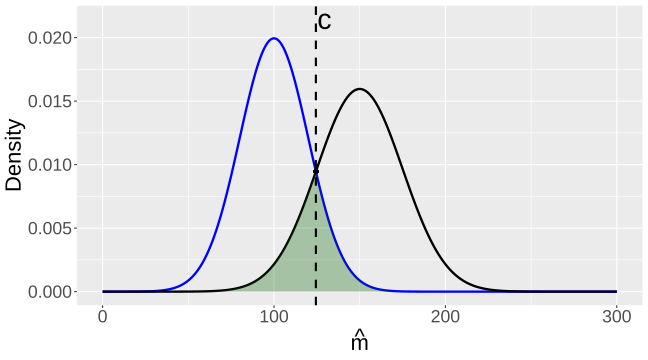
\includegraphics[width=0.8\linewidth]{plots/ovelappingarea.pdf}}
    \caption[Overlapping area of two normal distributions]{Overlapping area of two normal distributions. The point $c$ is the performance both distributions are equally likely to achieve. The shaded area denotes the probability of overlap between the two distributions; in our case, the probability that the candidate solver will perform as least as well as the best predicted solver.}
    \label{fig:overlappingarea}
\end{figure}

\section{Experimental Setup}
\subsection{Data Collection}

We used three scenarios from the ASlib benchmark repository ~\cite{BISCHL201641}: MAXSAT19-UCMS, SAT11-INDU, and SAT18-EXP. Additionally, we created two new scenarios: SAT16-MAIN, which utilizes solvers and instances from the SAT Competition 2016, and IPC2018, which incorporates solvers and instances from the International Planning Competition 2018. As ASlib only offers algorithm performance data for single runs, we conducted our own measurements for parallel runs on individual machines. We also measured the performance for single runs again and repeated the instance feature extraction steps to ensure that all experiments were performed on the same hardware. For MAXSAT19-UCMS, SAT11-INDU\footnote{For SAT11-INDU, the ASlib benchmark repository contains 115 extracted features, including those from SATZilla. However, we were unable to find the feature extraction for this scenario and used the same 54 instance features extracted by SATZilla.}, SAT16-MAIN, and SAT18-EXP, we used SATZilla’s feature computation code~\cite{satzilla}, and extracted 54 different features. For IPC2018 we used the feature extraction code by~\cite{Fawcett_Vallati_Hutter_Hoffmann_Hoos_Leyton-Brown_2014} which extracts 305 features for planning problems in PDDL format. We excluded 26 instances of SAT Competition 2016 from the SAT16-MAIN scenario because we were unable to extract features within two hours of computational time. 
We also omitted two solvers, glocusePLE and Scavel\_SAT, from SAT16-MAIN because of frequent out-of-memory errors on multiple instances. From IPC2018, we omitted three solvers, MSP, maplan-1, and maplan-2, because they require an unavailable version of CPLEX. Table~\ref{tab:scenarios} gives an overview of the scenarios, algorithms, instances, and features we use in our evaluation.

\begin{table}
\centering
\caption{Number of Algorithms, Instances, and Features Across All Scenarios.}
\label{tab:scenarios}
\begin{tabular}{p{5cm} cccc}
\toprule
Scenario & Algorithms & Instances & Instance Features\\
\midrule
IPC2018 & 15 & 240 & 305\\
MAXSAT19-UCMS & 7 & 572 & 54\\
SAT11-INDU & 14 & 300 & 54\\
SAT16-MAIN & 25 & 274 & 54\\
SAT18-EXP & 37 & 353 & 54\\
\bottomrule
\end{tabular}
\end{table}

We ran all solvers on all instances on compute nodes with 32 processors and 40 MB cache size (Intel(R) Xeon(R) CPU E5-2683 v4 @ 2.10GHz), 128 GB memory, and Red Hat Linux version 8.6. We use the same time limits as in the ASlib scenarios; 5000 CPU seconds for SAT18-EXP and SAT11-INDU, and 3600 CPU seconds for MAXSAT19-UCMS. For the new scenarios, we use the same time limits as the respective competitions; 5000 CPU seconds for SAT16-MAIN and 1800 CPU seconds for IPC2018. We ran each algorithm individually with 2-10 parallel runs. For all experiments, we ensured that only the given number of parallel runs were executed on a single machine. As our previous work showed that performance becomes worse than algorithm selection of a single solver for more than 10 parallel runs~\cite{pmlr-v140-kashgarani21a}, we did not evaluate more than 10 parallel runs.

\subsection{Training and Tuning}
In the paper ~\cite{kashgarani2023automatic}, we first built random forest regression models to predict the performance of an algorithm on an instance using LLAMA~\cite{LLAMA} and MLR~\cite{mlr}. To expand on the results of the paper, in addition to the initial performance model, we trained two additional algorithm selection performance models using the random forest implementation in the MLR3 package. We compared these with the previous randomForest model trained with the MLR package in R. 

MLR is an R package that unifies the available implementations of machine learning algorithms in R \cite{mlr}. In MLR, the Random Forests learner uses the randomForest package in R \cite{randomforest} as a dependency. The MLR package extends this algorithm by providing one method to estimate the uncertainties of the predictions, which is the Jackknife \cite{wager2014confidence} technique. MLR3 \cite{Bischl2024}, on the other hand, is the latest version of the MLR release, offering enhanced features. Some learners differ between MLR and MLR3. In MLR, training random forests uses the implementation of the randomForest R package, while MLR3 replaces this with the Ranger R package. According to its documentation, Ranger is designed to be a fast implementation of random forests, particularly for high-dimensional data \cite{ranger}. In Ranger's paper \cite{ranger} it outperforms other implementations, including randomForest, in terms of runtime and memory usage, especially as the number of trees, features, and sample sizes increases, and Ranger scaled almost linearly with the number of samples, while randomForest scaled superlinearly \cite{ranger}. 

Our MLR regression random forest models predict the runtime for each solver as the mean of the underlying distribution, and estimate the standard deviation using the Jackknife method~\cite{wager2014confidence,mlr}, which calculates the standard deviation of the mean predictions over all observations used to train the random forest. The random forest is trained on $n-1$ observations and makes a prediction for the remaining observation. This process is repeated for all observations. The mean prediction for each tree is determined by averaging its predictions for the left-out observations. The Jackknife method assumes that the distribution of the predictions is normal, and their standard deviation is the uncertainty of the overall prediction.

Ranger allows two different methods to estimate prediction uncertainties \cite{wager2014confidence}: the Jackknife (also known as the jackknife-after-bootstrap) and the infinitesimal Jackknife (also known as the infinitesimal-jackknife-for-bagging). We built random forest regression models using the Ranger package twice: one model with the Jackknife method (RJ) to estimate prediction uncertainty and the other with the Infinitesimal Jackknife method (RI).

The Jackknife and infinitesimal Jackknife methods both estimate the standard deviation, but differ in approach and efficiency according to \cite{wager2014confidence}. The jackknife removes one observation at a time to assess the impact, while the infinitesimal jackknife downweights each observation by an infinitesimal amount. So, the infinitesimal Jackknife method downweights each observation by a very small amount. This approach often leads to more stable predictions and is more computationally efficient, as it requires fewer bootstrap replicates for similar accuracy \cite{wager2014confidence}.

Random forests usually result in the best algorithm selection performance and performance predictions~\cite{BISCHL201641,HUTTER201479}.
Our setup mirrors that of~\cite{BISCHL201641}:  we removed constant-valued instance features and imputed missing feature values with the mean of all non-missing values for that feature. The
hyperparameters of the random forest models were tuned using random search with 250 iterations, with $ntree$ ranging from 10 to 200 and $mtry$ from 1 to 30 in a nested cross-validation with three
inner folds and 10 outer folds~\cite{BISCHL201641}.

Since the available version of LLAMA \cite{LLAMA} was only adapted to MLR, we ported the LLAMA package to MLR3 to conduct experiments and compare different implementations\footnote{https://github.com/uwyo-mallet/llama-mlr3}. This update will be available to the community in the near future as CRAN R package. 

To determine the optimal value of $p_{\cap}$ in Equation~\ref{eq:6} for each scenario, we perform a grid search in the $[0, 1)$ interval with a resolution of $0.01$ for a total of 100 values. Additionally, we determine the overall optimal value of $p_{\cap}$ across all five scenarios.

We evaluate the proposed approach using penalized average runtime with a factor of 10 (PAR10), misclassification penalty (MCP), runtime. The PAR10 score is equal to the actual runtime when the algorithm succeeds in solving the instance within the timeout, otherwise, it is the timeout times 10. The misclassification penalty is the difference between the performance of the selected algorithm and the performance of the optimal algorithm. We report the mean and standard deviation of these values in Tables~\ref{tab:summary},~\ref{tab:summary2}, and~\ref{tab:summary2}. 

We also measure the PAR10 score normalized gap closed between the sequential single best solver and the sequential virtual best solver. In Tables~\ref{tab:summary},~\ref{tab:summary2}, and~\ref{tab:summary2}, we report the mean and standard deviation of the normalized gap closed across the 10 folds of data used to train the performance models. In contrast to the reported runtime, MCP and PAR10 scores, in these tables, we do not report the mean and standard deviation in the distribution of all instances. Instead, we use folds because, based on the normalized gap closed formula $\frac{\text{sbs} - \text{approach}}{\text{sbs} - \text{vbs}}$, we aimed to avoid zero denominators in cases where the single best solver is the actual best solver for an instance. The plots~\ref{fig:all_results}, show the PAR10 score normalized gap closed over the entire distribution of instances.


\subsection{Baselines}

We compare the performance of our approach to several baseline methods, in particular the sequential virtual best solver (VBS), which is the optimal algorithm from the portfolio per problem instance (with a cumulative misclassification penalty of zero) and the sequential single best solver (SBS), which is the algorithm from the portfolio with the best average performance across all problem instances. The VBS for parallel runs is the best solver for each instance, but including the overhead for $n$ parallel runs. The parallel SBS is computed similarly, with the best solvers on average instead of the best on each instance. We run multiple solvers in parallel to measure the actual runtime of the best solver in this case, rather than assuming the sequential runtime.

We further compare to per-instance algorithm selection that simply runs the top $n$ predicted algorithms in parallel without considering the overlap of the distributions of the performance predictions, with the same performance models we use for our approach. In the notation we introduced above, we set $p_{\cap}=0$ and cap the number of runs at the number of available processors. 
We use a simple scheduling method as a further baseline, where algorithms are scheduled according to their predicted rank and allocated a time slice equal to the predicted performance plus the standard deviation. This allows to run more than one algorithm per processor. This approach prioritizes the best-predicted algorithms but also potentially allows other algorithms to run.

ASPEED~\cite{aspeed} provides a general schedule for all instances in a given scenario, rather than a schedule for each instance individually. Therefore, we do not include ASPEED in our experimental evaluation -- static schedules across large sets of problem instances do not achieve competitive performance, as shown in~\cite{flexfolio}. The Flexfolio paper~\cite{flexfolio} shows experiments for Instance-Specific ASPEED and TSunny, but the available source code does not contain these algorithm selection methods and we are unable to compare to them.

Finally, we compare our approach to 3S as implemented in Flexfolio~\cite{flexfolio}, as the original 3S implementation is unavailable. In this implementation, the number of neighbors for the kNN models was set to 32, and ASPEED~\cite{aspeed} is used to schedule the chosen solvers instead of the original integer programming scheduler.

We normalize all performances across scenarios by the performances of the VBS and SBS and report the fraction of the gap between them that was closed by a particular approach. On this normalized scale, 0 corresponds to the performance of the SBS and 1 to the performance of the VBS.
All code and data are available at \url{https://github.com/uwyo-mallet/auto-parallel-portfolio-selection}.

\section{Results}
\subsection{Tuning of $p_{\cap}$}

\begin{figure}[t]
\centering
    \includegraphics[width=0.48\linewidth]{plots/Theta_sensitivity_x_theta_y_runtime_facet.pdf}
    \includegraphics[width=.48\linewidth]{plots/pcap_ri_sensitivity_x_theta_y_runtime_facet.pdf}
    \includegraphics[width=.48\linewidth]{plots/pcap_rj_sensitivity_x_theta_y_runtime_facet.pdf}
    \caption[Sensitivity of portfolio performance to $p_{\cap}$]{Sensitivity of portfolio performance to $p_{\cap}$. The top-left plot refers to the RFJ model—Regression Random Forest model using MLR with the Jackknife uncertainty estimation method. The top-right plot refers to the RI model—Regression Ranger model with the Infinitesimal Jackknife uncertainty estimation method. The bottom plot refers to the RJ model—Regression Ranger model with the Jackknife uncertainty estimation method. The plot illustrates the mean, Q1 (25th percentile), Q2 (50th percentile), and Q3 (75th percentile) runtime performance of each scenario for various values of $p_{\cap}$ as defined in Equation~\ref{eq:7}. Note the log scale for the normalized gap closed.}
    \label{fig:sensitivity}
\end{figure}

The tuning of $p_{\cap}$ shows that the optimal value depends on the scenario. For the IPC2018 scenario, the ideal $p_{\cap}$ value is 0.59, for the MAXSAT19-UCMS scenario 0.55, for SAT11-INDU 0.63, for SAT16-MAIN 0.33, and for SAT18-EXP 0.81 for the random forest model trained using the MLR and Jackknife uncertainty estimation method (RFJ). The optimal $p_{\cap}$ values for the Ranger models, one with Jackknife (RJ) and the other with Infinitesimal Jackknife (RI), are provided in Table~\ref{tab:pcap}.

\begin{table}
\centering
\caption{Optimum value of $p_{\cap}$ for each benchmark and model.}
\label{tab:pcap}
\begin{tabular}{p{3.6cm} cccc}
\toprule
Scenario & RandomForest\_Jackknife & Ranger\_Jackknife & Ranger\_Inifinitesimal\\
\midrule
IPC2018 & 0.59 & 0.27 & 0.44 \\
MAXSAT19-UCMS & 0.55 & 0.14 & 0.03\\
SAT11-INDU & 0.63 & 0.31 & 0.01\\
SAT16-MAIN & 0.33 & 0.33 & 0\\
SAT18-EXP & 0.81 & 0.58 & 0.55\\
\midrule
Generic best & 0.82 & 0.31 & 0.17\\
\bottomrule
\end{tabular}
\end{table}


Figures~\ref{fig:sensitivity} shows the normalized gap closed for the mean, 25th percentile, 50th percentile, and 75th percentiles for each scenario depending on $p_{\cap}$. While the optimal values are very different across different scenario and each algorithm selector, the differences in terms of gap closed are relatively small as long as $p_{\cap}$ is not too large. The best average value for $p_{\cap}$ across all scenarios for RFJ model, RI model, and RJ model are 0.82, 0.17, 0.31 respectively which yields performance improvements over the baselines in most cases (see Table~\ref{tab:summary}). For the overall best performance, we recommend to tune $p_{\cap}$ for the particular scenario. However, using the generic best values of 0.82, 0.17, and 0.31 for RFJ, RI, and RJ, respectively, provides a reasonable starting point that yields good performance across the range of scenarios considered here.

The optimal value of $p_{\cap}$ allows us to draw conclusions with respect to the predictive accuracy of the performance models we are using. A small value would suggest that the predictions of the performance models are not very accurate, as we have to include even solvers whose predicted runtime distribution has a small overlap with the runtime distribution of the best predicted solver to include solvers that are actually good. If the optimal value of $p_{\cap}$ was 0, we would have to include all solvers, even the ones whose predicted distribution has no overlap with the best predicted solver -- in other words, the predicted runtime distribution of the actual best solver has no overlap with the predicted runtime distribution of the best predicted solver. 

Here, for the RFJ model, the optimal values for $p_{\cap}$ are relatively large in most cases, and even the smallest values are far greater than 0. For the RJ model, the values are lower than those for the RFJ model, except for SAT16-MAIN, where the values are equal. For the RI model, except for IPC2018, the values are even lower than those for the RJ model. This indicates that the predictions of the performance models for RFJ are quite good -- while the best predicted solver is not always the actual best solver for a given problem instance, the predicted runtime distribution of the actual best solver has a large overlap with the predicted runtime distribution of the predicted best solver. 

Based on the low values of the RI model, it appears that this model performs worse than the other two. This claim is also evident in Table~\ref{tab:summary} where, for IPC2018, MAXSAT19-UCMS, and SAT11-INDU, the performance of the $AS$ (RI) model is worse than the other two in at least two of the performance measurements. For SAT16-MAIN, the $AS$ (RI) model performs worst only in terms of PAR10, indicating more timeouts; however, on average, it provides better runtime predictions, so the runtime and MCP measures are better than those of the RJ model. For SAT18-EXP, as shown in Table~\ref{tab:pcap}, the RI model has a slightly lower $p_{\cap}$ value than the RJ model; however, the difference is minimal, and the RI model performs better than the RJ model according to Table~\ref{tab:summary}. Overall, according to Table~\ref{tab:summary}, the RFJ model outperforms the other two models in at least two performance metrics in 4 out of 5 scenarios when performing single algorithm selection.

\subsection{Algorithm Selection Results}
\begin{figure}
        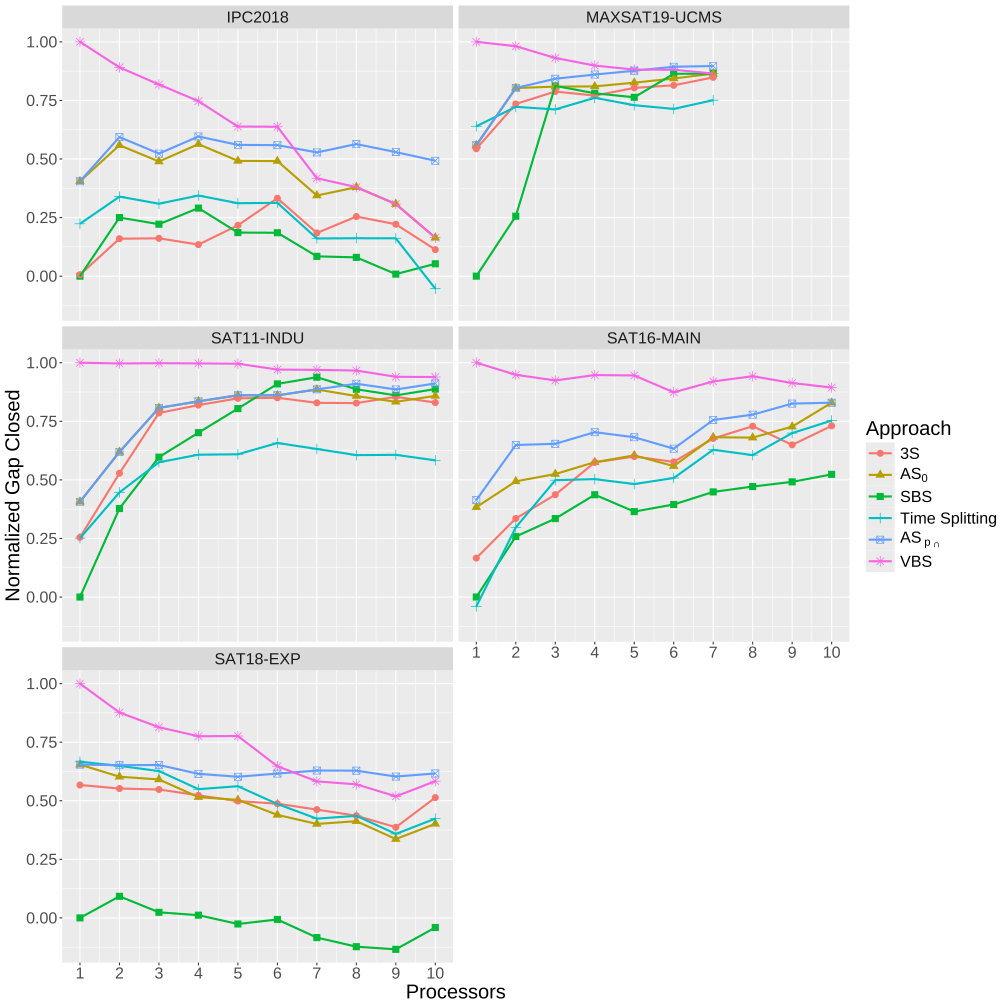
\includegraphics[width=\linewidth]{plots/line_chart_parallel_NormalizedGap_2col.pdf}    
    \caption[Results Summary: Comparing $AS_{p_{\cap}}$ with Baselines]{
    Summary of results. The plot shows the degree to which the gap between the SBS and VBS PAR10 scores is closed by each method. For the VBS and SBS, we choose the top $n$ solvers, where $n$ is the number of processors, for a given problem instance and across all instances, respectively. $AS_0$ chooses the top $n$ solvers predicted by algorithm selection, without regard for any overlap in their predicted runtime distributions. $AS_{p_{\cap}}$ represents the proposed formulation, with the number of processors restricted to at most the specific value indicated on the x axis -- depending on the overlap of the predicted runtime distributions, fewer solvers than the maximum may be chosen. The $p_{\cap}$ values for IPC2018, MAXSAT19-UCMS, SAT11-INDU, SAT18-EXP, and SAT16-MAIN are 0.59, 0.55, 0.63, 0.81, and 0.33 and respectively. Time Splitting is the baseline approach that allocates time proportional to the predicted runtime and standard deviation for each solver, scheduling more than one solver to be run per processor.}
    \label{fig:all_results}
\end{figure}

\begin{figure}
    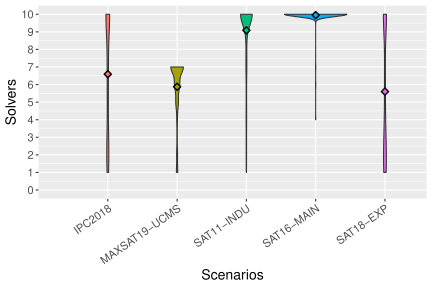
\includegraphics[width=0.5\linewidth]{plots/x_Scenario_y_Solver.pdf}
    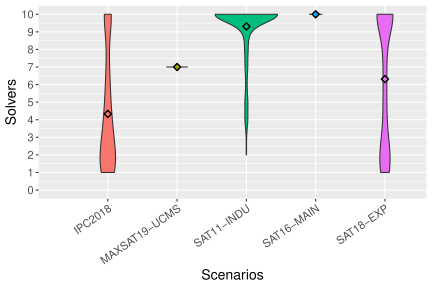
\includegraphics[width=0.5\linewidth]{plots/number_of_solvers_infjack_pcap.pdf}
    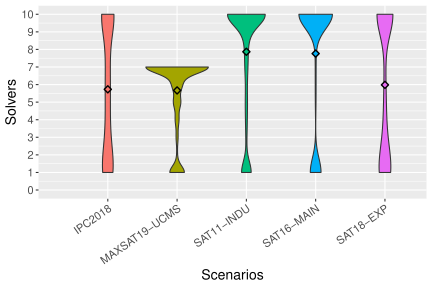
\includegraphics[width=0.5\linewidth]{plots/number_of_solvers_jack_pcap.pdf}

    \caption[Distribution of Number of Selected Solvers when Using $AS_{p_{\cap}}$]{
    Violin plot of the distribution of the number of selected solvers to run in parallel across all problem instances for each scenario for the respective optimal $p_{\cap}$ and the maximum level of parallelism (seven processors for MAXSAT19-UCMS and 10 for all other scenarios). The diamond denotes the mean value. The top-left plot refers to the RFJ model, the top-right plot to the RI model, and the bottom plot to the RJ model.
    }
    \label{fig:x_Scenario_y_Solver}
\end{figure}

To evaluate the effectiveness of our approach, we carried out a series of experiments using the optimum and the average best value for $p_{\cap}$ for each scenario using the RFJ model where we varied the number of processors used for parallel execution from one to ten for the SAT18-EXP, SAT16-MAIN, SAT11-INDU, and IPC2018 scenarios. For the MAXSAT19-UCMS scenario, we used a maximum of seven processors as there are only seven algorithms. For RFJ model Figure~\ref{fig:all_results} shows the PAR10 score results in terms of the normalized performance gap between the sequential single best solver and sequential virtual best solver for all scenarios and numbers of processors.

The figure demonstrates the promise of the approach we propose here. In three out of five scenarios, we achieve the overall top performance with the maximum number of processors (even better than the parallel virtual best solver!) and for the remaining two scenarios only the parallel virtual best solver is better. We are able to achieve better performance than the parallel virtual best solver when running in parallel because our approach does not necessarily use all available processors, unlike the baseline approaches that we compare to. While the performance of the virtual best solver suffers for a large number of parallel runs, our approach keeps the overhead of running many things in parallel low and is thus better overall. We emphasize that the results we show here are actual measured values for running in parallel, rather than assuming overhead-free parallelization based on sequential runtimes, as is commonly done in the literature. Our results demonstrate that this common assumption is unrealistic except for a small number of parallel runs.

Even for a small number of processors, our approach yields better performance than others. Initially, the performance is similar to $AS_0$ (running the top $n$ solvers), but our approach quickly becomes better as the number of available processors increases. This is expected, as for a single processor the two methods run exactly the same solver, but for a larger number of processors our method may not run as many as $AS_0$, thus decreasing overhead and overall solving performance.

For the IPC2018 scenario, we achieve the best overall results, improving performance substantially over all other approaches for 10 processors. The 3S approach is never close to the performance of our method and consistently yields worse results. The greedy time-splitting method also underperformed, often allocating time slices smaller than required to solve the instance and thus wasting resources. For more than seven parallel runs, the parallel virtual best solver, i.e.\ choosing the actual best solvers for each instance to run in parallel, starts to perform worse than our method, which does not use as many processors and incurs lower overhead.

The results for the other scenarios are qualitatively similar. While for a small number of processors, other methods perform similar to ours, the gap between them widens as the number of parallel runs increases. 3S consistently shows worse performance, whereas running the top $n$ solvers based on algorithm selection (without considering the predicted performance distributions) is usually competitive and in some cases gives the same performance as our method. The baseline of allocating a time to run proportional to the predicted runtime and standard deviation for each solver is not competitive, consistently showing bad performance -- this baseline is worse than simply running the top $n$ single best solvers in parallel on three scenarios for large numbers of parallel runs. For the IPC2018 and MAXSAT19-UCMS scenarios, the performance of some methods becomes worse than the single best solver for large numbers of processors, showing the limitations of these approaches. For the SAT2016-MAIN scenario, our approach is performing so close to the na\"ive parallel algorithm selection (top $n$ solvers based on algorithm selection) because the standard error of the predictions was large and this resulted in large parallel portfolios for the majority of instances.

Table~\ref{tab:summary} shows more detailed results. The normalized gap closed represented the mean and standard deviation of the normalized gap closed across the 10 folds, whereas the ~\ref{fig:all_results} shows the mean of the normalized gap closed across all instances at once. We see that our method results in substantial savings in terms of all three measures across all scenarios -- the proposed approach is always the best overall, regardless of the performance measure. Note that we never beat the sequential VBS, which represents the upper bound on the performance of any algorithm selection system -- we cannot do better than only running the actual best solver. In many cases, the actual performance we achieve is close to the sequential VBS though. The results also show that using the ``generic'' best value for $p_{\cap}$ of 0.82 still gives substantial performance improvements over other approaches -- usually it gives the second best performance. The only exception to this are the MAXSAT19-UCMS and SAT2016-MAIN scenarios, where running the top $n$ solvers predicted by algorithm selection does better. The gap is relatively small though, and we still beat most of the other baselines.

\begin{table}[t]
\begin{center}
    {\caption[Detailed Results: Runtime, MCP, PAR10, and Normalized Gap Closed for $AS_{p_{\cap}}$ vs. Baselines PC2018 and MAXSAT19-UCMS Scenarios]{Detailed results. Mean and standard deviation of values for runtime, MCP, and PAR10 across all problem instances in a scenario for the sequential virtual best solver, sequential single best solver, and single top predicted algorithm in the initial three rows. The second set of rows for each scenario shows the results for the maximum number of processors (10 for IPC2018, and 7 for MAXSAT19-UCMS) for our approach and the baselines we compare to. All numbers were rounded to integers. The best value for each scenario and measure is shown in \textbf{bold} (excepting the sequential VBS, which is by definition always the best), the second best in \textit{italics}. The normalized gap closed represents the mean and standard deviation of the normalized gap closed across the folds.}\label{tab:summary}}
    \scriptsize\begin{tabular}{clcccc}
    \toprule
        Scenario & Approach & Runtime [s] & MCP & PAR10 & NormalizedGap\\
    \midrule
    
    \multirow{17}{*}{\rotatebox{90}{IPC2018}} & \multicolumn{5}{c}{\textbf{1 Processor}} \\\cmidrule{2-6}
        & VBS & 508$\pm$697 & 0 & 3478$\pm$6903 & 1\\
        & AS (RFJ) & 607$\pm$751 & 99$\pm$301 & 4657$\pm$7725 & -0.44$\pm$2.84\\
        & AS (RI) & 608$\pm$751 & 100$\pm$293 & 4456$\pm$7583 & -0.35$\pm$2.85\\
        & AS (RJ) & 604$\pm$752 & 96$\pm$293 & 4519$\pm$7633 & -0.39$\pm$2.84 \\
        & SBS & 734$\pm$770 & 226$\pm$414 & 5459$\pm$8072 & 0 \\
    \cmidrule{2-6}  
    & \multicolumn{5}{c}{\textbf{10 Processors}}\\
    \cmidrule{2-6}
        %& VBS &  &  &  \\
        %& SBS &  &  & \\
        & 3S & 645$\pm$770 & 137$\pm$471 & 5235$\pm$8047 & -0.76$\pm$2.7\\
        & Time Splitting (RFJ) & 637$\pm$797 & 129$\pm$348 & 5565$\pm$8241 & -0.84$\pm$2.5\\
        & Time Splitting (RI) & 641$\pm$799 & 133$\pm$361 & 5636$\pm$8274 & -0.99$\pm$2.52\\
        & Time Splitting (RJ) & 636$\pm$794 & 128$\pm$353 & 5496$\pm$8206 &  -0.92$\pm$2.51\\
        & $AS_0$ (RFJ) & 612$\pm$779 & 104$\pm$307 & 5134$\pm$8027 & -0.66$\pm$2.56\\
        & $AS_0$ (RI)  & 616$\pm$783  & 107$\pm$312 & 5206$\pm$8065 & -0.69$\pm$2.54\\
        & $AS_0$ (RJ)  & 616$\pm$783 & 107$\pm$312 & 5206$\pm$8065 & -0.69$\pm$2.54 \\ 
        & $AS_{p_{\cap} = 0.59}$ (RFJ) & \emph{569$\pm$745} & \emph{61$\pm$223} & 4484$\pm$7651 & \textbf{-0.18$\pm$2.74} \\
        & $AS_{p_{\cap} = 0.44}$ (RI) & \textbf{557$\pm$728} & \textbf{49$\pm$190} & \textbf{4135$\pm$7403} & \emph{-0.19$\pm$2.89}\\
        & $AS_{p_{\cap} = 0.27}$ (RJ) & 570$\pm$744 & 62$\pm$229 & 4350$\pm$7552 &  -0.21$\pm$2.72 \\
        & $AS_{p_{\cap} = 0.82}$ (RFJ) & 579$\pm$742 & 70$\pm$233 & 4359$\pm$7548  & -0.26$\pm$2.88 \\
        & $AS_{p_{\cap} = 0.17}$ (RI) & 570$\pm$739 & 62$\pm$230 & \emph{4283$\pm$7501} & -0.24$\pm$2.87\\
        & $AS_{p_{\cap} = 0.31}$ (RJ) & 570$\pm$743 & 62$\pm$229 & 4350$\pm$7552 & -0.21$\pm$2.72\\
    \midrule
    \multirow{19}{*}{\rotatebox{90}{MAXSAT19-UCMS}} & \multicolumn{5}{c}{\textbf{1 Processor}} \\\cmidrule{2-6}
        & VBS & 858$\pm$1476 & 0 & 7768$\pm$14717 & 1\\
        & AS (RFJ) & 1037$\pm$1555 & 179$\pm$641 & 9363$\pm$15684 & 0.55$\pm$0.28\\
        & AS (RI) & 1076$\pm$1575 & 218$\pm$729 & 9686$\pm$15850 & 0.45$\pm$0.34 \\
        & AS (RJ) & 1044$\pm$1565 & 186$\pm$666 & 9540$\pm$15793 & 0.49$\pm$0.23 \\
        & SBS & 1190$\pm$1657 & 332$\pm$940 & 11386$\pm$16696 & 0 \\
    \cmidrule{2-6}   
    & \multicolumn{5}{c}{\textbf{7 Processors}}\\
    \cmidrule{2-6}  
        %& VBS & 894.42 & 37.11 & 8258.05 \\
        %& SBS & 894.42 & 37.11 & 8258.05\\
        & 3S & 953$\pm$1480 & 95$\pm$437 & 8317$\pm$15031 & 0.83$\pm$0.16 \\
        & Time Splitting (RFJ) & 908$\pm$1523 & 51$\pm$308 & 8668$\pm$15353 & 0.75$\pm$0.16 \\
        & Time Splitting (RI) & 919$\pm$1535 & 61$\pm$356 & 8849$\pm$15470  & 0.7$\pm$0.2\\
        & Time Splitting (RJ) & 917$\pm$1531 & 59$\pm$352 & 8790$\pm$15431 & 0.71$\pm$0.2 \\
        & $AS_0$ (RFJ) & \emph{894$\pm$1506} & \emph{37$\pm$247} & 8258$\pm$15062 & 0.85$\pm$0.16\\
        & $AS_0$ (RI) & \emph{894$\pm$1506} & \emph{37$\pm$247} & 8258$\pm$15062 & 0.85$\pm$0.16 \\ 
        & $AS_0$ (RJ) & \emph{894$\pm$1506} & \emph{37$\pm$247} & 8258$\pm$15062 & 0.85$\pm$0.16\\
        & $AS_{p_{\cap} = {0.55}}$ (RFJ) & \textbf{891$\pm$1496} & \textbf{33$\pm$215} & \textbf{8141$\pm$14975} & \textbf{0.88$\pm$0.17} \\
        & $AS_{p_{\cap} = 0.03}$ (RI) & \emph{894$\pm$1506} & \emph{37$\pm$247} & 8258$\pm$15062 & 0.85$\pm$0.16  \\ 
        & $AS_{p_{\cap} = 0.14}$ (RJ) & 921$\pm$1521 & 63$\pm$369 & 8568$\pm$15263 &  0.76$\pm$0.24 \\
        & $AS_{p_{\cap} = 0.82}$ (RFJ) & 928$\pm$1513 & 70$\pm$364 & 8461$\pm$15175 & 0.81$\pm$0.18\\
        & $AS_{p_{\cap} = 0.17}$ (RI) & 901$\pm$1502 & 43$\pm$275 & \emph{8208$\pm$15015} &  \textbf{0.88$\pm$0.16} \\
        & $AS_{p_{\cap} = 0.31}$ (RJ) & 931$\pm$1525 & 73$\pm$402 & 8578$\pm$15259 & 0.78$\pm$0.21 \\
\bottomrule
    \end{tabular}    
\end{center}
\end{table}


\begin{table}[t]
\begin{center}
    {\caption[Detailed Results: Runtime, MCP, PAR10, and Normalized Gap Closed for $AS_{p_{\cap}}$ vs. Baselines for SAT11-INDU and SAT16-MAIN Scenar]{Detailed results. Mean and standard deviation of values for runtime, MCP, and PAR10 across all problem instances in a scenario for the sequential virtual best solver, sequential single best solver, and single top predicted algorithm in the initial three rows. The second set of rows for each scenario shows the results for the maximum number of processors (10 for SAT16-MAIN and SAT11-INDU) for our approach and the baselines we compare to. All numbers were rounded to integers. The best value for each scenario and measure is shown in \textbf{bold} (excepting the sequential VBS, which is by definition always the best), the second best in \textit{italics}. The normalized gap closed represents the mean and standard deviation of the normalized gap closed across the folds.}\label{tab:summary2}}
    \scriptsize\begin{tabular}{clcccc}
    \toprule
        Scenario & Approach & Runtime [s] & MCP & PAR10 & NormalizedGap\\
    \midrule
    \multirow{17}{*}{\rotatebox{90}{SAT11-INDU}} & \multicolumn{5}{c}{\textbf{1 Processor}} \\\cmidrule{2-6}
        & VBS & 1140$\pm$1836 & 0 & 8040$\pm$17905 & 1\\
        & AS (RFJ) & 1535$\pm$2058 & 395$\pm$1037 & 11735$\pm$20768 & 0.16$\pm$0.79\\        
        & AS (RI) & 1610$\pm$2108 & 470$\pm$1145 & 12710$\pm$21389 & -0.06$\pm$0.9\\
        & AS (RJ) & 1565$\pm$2049 & 425$\pm$1017 & 11315$\pm$20402 & 0.34$\pm$0.49\\
        & SBS & 1818$\pm$2168 & 678$\pm$1340 & 14268$\pm$22154 & 0 \\
    \cmidrule{2-6}    
    & \multicolumn{5}{c}{\textbf{10 Processors}}\\
    \cmidrule{2-6}    
        %& VBS &  &  &  \\
        %& SBS &  &  &  \\
        & 3S & 1298$\pm$1898 & 158$\pm$546 & 9098$\pm$18780 & 0.78$\pm$0.3\\
        & Time Splitting (RFJ) & 1335$\pm$2009 &  225$\pm$708 & 10635$\pm$20138 & 0.49$\pm$0.61 \\
        & Time Splitting (RI) & 1429$\pm$2108 & 318$\pm$875 & 12379$\pm$21378 & 0.19$\pm$0.53\\
        & Time Splitting (RJ) & 1334$\pm$1998 & 224$\pm$689 & 10634$\pm$20138 & 0.55$\pm$0.43 \\
        & $AS_0$ (RFJ) & 1272$\pm$1927 & 161$\pm$548 & 8922$\pm$18645 & \emph{0.89$\pm$0.12}\\
        & $AS_0$ (RI) & \emph{1238$\pm$1892} & 127$\pm$385 & \emph{8588$\pm$18350} & \textbf{0.92$\pm$0.1}\\ 
        & $AS_0$ (RJ) & 1262$\pm$1910 & 151$\pm$480 & 8612$\pm$18342 & \textbf{0.92$\pm$0.1} \\
        & $AS_{p_{\cap} = 0.63}$ (RFJ) & 1241$\pm$1901 & 131$\pm$451 & 8591$\pm$18349 & \textbf{0.92$\pm$0.1} \\
        & $AS_{p_{\cap} = 0.01}$ (RI) & \textbf{1236$\pm$1890} & \textbf{121$\pm$379} & \textbf{8586$\pm$18351} & \textbf{0.92$\pm$0.1} \\ 
        & $AS_{p_{\cap} = 0.31}$ (RJ) & 1289$\pm$1934 & 178$\pm$595 & 9089$\pm$18787 & 0.78$\pm$0.28\\
        & $AS_{p_{\cap} = 0.82}$ (RFJ) & 1247$\pm$1900 & \emph{123$\pm$431} & 8747$\pm$18501 &  0.83$\pm$0.28 \\
        & $AS_{p_{\cap} = 0.17}$ (RI) & 1259$\pm$1912 & 139$\pm$477 & 8909$\pm$18649 & 0.74$\pm$0.36\\
        & $AS_{p_{\cap} = 0.31}$ (RJ) & 1289$\pm$1934 & 178$\pm$595 & 9089$\pm$18787 & 0.78$\pm$0.28 \\
    \midrule 
    \multirow{19}{*}{\rotatebox{90}{SAT16-MAIN }} & \multicolumn{5}{c}{\textbf{1 Processor}} \\\cmidrule{2-6}
        & VBS & 1867$\pm$2193 & 0 & 15005$\pm$22530 & 1\\
        & AS (RFJ) & 2315$\pm$2273 & 448$\pm$1109 & 19066$\pm$23883 & 0.33$\pm$0.56\\
        & AS (RI) & 2383$\pm$2294 & 516$\pm$1151 & 19956$\pm$24111 & 0.05$\pm$0.66\\ 
        & AS (RJ) & 2400$\pm$2269 & 533$\pm$1177 & 19316$\pm$23880 & 0.3$\pm$0.24\\ 
        & SBS & 2560$\pm$2294 & 693$\pm$1415 & 21940$\pm$24464 & 0\\
    \cmidrule{2-6}
    & \multicolumn{5}{c}{\textbf{10 Processors}}\\
    \cmidrule{2-6}
        %& VBS &  1944.82 & 78.13 & 15740.44\\
        %& SBS & 2214.08 & 347.38 & 18308.97\\
        & 3S & 2093$\pm$2228 & 226$\pm$547 & 16874$\pm$23228 & 0.59$\pm$0.59\\
        & Time Splitting (RFJ) & 2101$\pm$2247 & 234$\pm$732 & 16717$\pm$23149 & \textbf{0.78$\pm$0.46} \\
        & Time Splitting (RI) & 2089$\pm$2256 & 222$\pm$642 & 17691$\pm$23593 & 0.37$\pm$0.85\\
        & Time Splitting (RJ) & 2098$\pm$2254 & 231$\pm$674 & 17372$\pm$23447 & 0.56$\pm$0.39\\
        & $AS_0$ (RFJ) & 2065$\pm$2221 & 198$\pm$652 & \textbf{16189$\pm$22931} & \emph{0.7$\pm$0.39}\\
        & $AS_0$ (RI)& \textbf{2016$\pm$2225} & \textbf{150$\pm$503} & 16469$\pm$23122 & 0.68$\pm$0.6\\ 
        & $AS_0$ (RJ)& 2048$\pm$2228 & 181$\pm$597 & \emph{16336$\pm$23023} & 0.68$\pm$0.59\\ 
        & $AS_{p_{\cap} = 0.33}$ (RFJ) & 2065$\pm$2221 & 198$\pm$652 & \textbf{16189$\pm$22931} & \emph{0.7$\pm$0.39}\\
        & $AS_{p_{\cap} = 0}$ (RI) & \textbf{2016$\pm$2225} & \textbf{150$\pm$503} & 16469$\pm$23122 & 0.68$\pm$0.6\\ 
        & $AS_{p_{\cap} = 0.33}$ (RJ) & 2088$\pm$2239 & 222$\pm$704  & 16705$\pm$23156 & 0.64$\pm$0.37\\ 
        & $AS_{p_{\cap} = 0.82}$ (RFJ) & 2094$\pm$2222 & 228$\pm$730 & 16383$\pm$22993 & 0.69$\pm$0.41\\
        & $AS_{p_{\cap} = 0.17}$ (RI) & \emph{2041$\pm$2230} & \emph{174$\pm$591} & 16822$\pm$23261 & 0.57$\pm$0.63\\
        & $AS_{p_{\cap} = 0.31}$ (RJ) & 2096$\pm$2240 & 229$\pm$713 & 16877$\pm$23227 & 0.63$\pm$0.36\\  
        \bottomrule
    \end{tabular}    
\end{center}
\end{table}
\begin{table}[t]
\begin{center}
    {\caption[Detailed Results: Runtime, MCP, PAR10, and Normalized Gap Closed for $AS_{p_{\cap}}$ vs. Baselines for SAT18-EXP Scenario]{Detailed results. Mean and standard deviation of values for runtime, MCP, and PAR10 across all problem instances in a scenario for the sequential virtual best solver, sequential single best solver, and single top predicted algorithm in the initial three rows. The second set of rows for each scenario shows the results for the maximum number of processors (10 for SAT18-EXP) for our approach and the baselines we compare to. All numbers were rounded to integers. The best value for each scenario and measure is shown in \textbf{bold} (excepting the sequential VBS, which is by definition always the best), the second best in \textit{italics}. The normalized gap closed represents the mean and standard deviation of the normalized gap closed across the folds.}\label{tab:summary3}}
    \scriptsize\begin{tabular}{clcccc}
    \toprule
        Scenario & Approach & Runtime [s] & MCP & PAR10 & NormalizedGap\\
    \midrule    
    \multirow{19}{*}{\rotatebox{90}{SAT18-EXP }} & \multicolumn{5}{c}{\textbf{1 Processor}} \\\cmidrule{2-6}
         & VBS & 1146$\pm$1945 & 0 & 9687$\pm$19547 & 1\\
         & AS (RFJ) & 1615$\pm$2138 & 468$\pm$1192 & 13470$\pm$21889 & 0.64$\pm$0.18\\
         & AS (RI) & 1648$\pm$2151 & 502$\pm$1256 & 13758$\pm$22034 & 0.59$\pm$0.18\\
         & AS (RJ) & 1690$\pm$2170 & 543$\pm$1302 & 14183$\pm$22247 & 0.57$\pm$0.16\\
         & SBS & 2400$\pm$2249 & 1254$\pm$1832 & 20629$\pm$24280 & 0\\
    \cmidrule{2-6}    
    & \multicolumn{5}{c}{\textbf{10 Processors}}\\
    \cmidrule{2-6}    
         %& VBS & 1496.22 & 350.06 & 14244.10 \\
         %& SBS & 2210.87 & 1064.70 & 21077.73 \\
         & 3S & 1625$\pm$2228 & 479$\pm$1265 & 15010$\pm$22802 & 0.5$\pm$0.23\\
         & Time Splitting (RFJ) & 1714$\pm$2292 & 571$\pm$1384 & 15992$\pm$23222 & 0.42$\pm$0.23\\
         & Time Splitting (RI) & 1640$\pm$2266 & 497$\pm$1280 & 15408$\pm$23003 & 0.46$\pm$0.24\\
         & Time Splitting (RJ) & 1745$\pm$2308  & 602$\pm$1434 & 16151$\pm$23267 & 0.4$\pm$0.24\\
         & $AS_0$ (RFJ) & 1702$\pm$2301 & 559$\pm$1389 & 16235$\pm$23355 & 0.39$\pm$0.27\\
         & $AS_0$ (RI) & 1654$\pm$2285 & 511$\pm$1324 & 15804$\pm$23194 & 0.42$\pm$0.29\\
         & $AS_0$ (RJ) & 1678$\pm$2288 & 535$\pm$1351 & 15956$\pm$23243 & 0.4$\pm$0.3 \\
         & $AS_{p_{\cap} = 0.81}$ (RFJ) & \textbf{1518$\pm$2172} & \textbf{372$\pm$1124} & \textbf{13884$\pm$22265} & \textbf{0.62$\pm$0.22} \\
         & $AS_{p_{\cap} = 0.55}$ (RI) & 1541$\pm$2191 & 397$\pm$1177 & 14034$\pm$22332 & \emph{0.6$\pm$0.21}\\ 
         & $AS_{p_{\cap} = 0.58}$ (RJ) & 1622$\pm$2237 & 477$\pm$1268 & 15008$\pm$22805 & 0.5$\pm$0.25\\
         & $AS_{p_{\cap} = 0.82}$ (RFJ) & \emph{1532$\pm$2178} & \emph{386$\pm$1146} &  \emph{14025$\pm$22336} & \emph{0.6$\pm$0.23}\\
         & $AS_{p_{\cap} = 0.17}$ (RI) & 1555$\pm$2221 & 410$\pm$1191 & 14558$\pm$22628 & 0.57$\pm$0.23\\
         & $AS_{p_{\cap} = 0.31}$ (RJ) & 1649$\pm$2265 & 505$\pm$1319 & 15544$\pm$23064 & 0.46$\pm$0.26\\
    \bottomrule
    \end{tabular}    
\end{center}
\end{table}
\subsection{Number of Selected Solvers}

As mentioned above, allowing our approach to use up to a certain number of processors does not mean that this exact number of parallel runs will be done. In practice, it is often much lower than that, as we see when comparing the performance of our approach to $AS_0$, which runs the top $n$ predicted solvers in parallel. Figure~\ref{fig:x_Scenario_y_Solver} shows the distribution of the number of selected solvers for each scenario and each algorithm selector. For RFJ, the mean number of solvers chosen for IPC2018 is around 6.5, for MAXSAT19-UCMS around 6 (out of 7), for SAT11-INDU around 9, for SAT16-MAIN around 10, and for SAT18-EXP around 5.5. For RI, the mean number of solvers chosen for IPC2018 is around 4.5, for MAXSAT19-UCMS around 7 (out of 7), for SAT11-INDU around 9.5, for SAT16-MAIN around 10, and for SAT18-EXP around 6.5. Similarly, for RJ, the mean number of solvers chosen for IPC2018 is around 6, for MAXSAT19-UCMS around 6 (out of 7), for SAT11-INDU around 8, for SAT16-MAIN around 8, and for SAT18-EXP around 6. 

For RFJ, we see that the largest difference to the maximum number of parallel runs occurs for the two scenarios where we observe the largest performance improvements of our approach, IPC2018 and SAT18-EXP. Similarly, the scenario with the highest number of solvers chosen on average (SAT16-MAIN) is where we see the smallest performance improvement. For RI and RJ the same comparison also exists. This clearly shows again that the advantage of our approach is that it does not simply use as many parallel processors as are available, which increases overhead, but intelligently chooses how many of the available processors to use for best performance. In at least some cases, more is less, and we show how to leverage this.

Figure~\ref{fig:x_Scenario_y_Solver} also shows that our approach uses the full range of available parallel runs in most cases, from running only a single solver to as many parallel runs as there are processors. Our approach is not simply a one-size-fits all that usually uses a similar number of runs, but varies the size of the selected parallel portfolio dynamically, based on the instance to be solved.

\subsection{Ranger vs RandomForest Results}
Figure~\ref{fig:rangervsrf} presents a comparison between the random forest implementation and the ranger implementations. When comparing the naive algorithm selection methods $AS (RFJ)$, $AS (RJ)$ and $AS (RI)$, which select the best predicted algorithm, based on Tables~\ref{tab:summary},~\ref{tab:summary2} and~\ref{tab:summary3}, the RFJ model emerges as a more promising algorithm selector in all scenarios except IPC2018, where the RJ model performs slightly better in terms of runtime and MCP. For SAT11-INDU, the $AS (RFJ)$ method is superior in terms of runtime and MCP, but performs slightly worse than the RI model in terms of PAR10.

When we compare $AS_{0} (RFJ)$, $AS_{0} (RJ)$, and $AS_{0} (RI)$, which select the top predicted algorithms to run in parallel, the performance of these methods is very competitive. In some cases, the RI model performs better, such as in SAT18-EXP and SAT11-INDU, across all metrics, and is superior only in terms of runtime and MCP in SAT16-MAIN. In other cases, the RFJ model performs better, as seen in IPC2018. For MAXSAT19-UCMS, all algorithm selectors perform equally, as with $p_{\cap} = 0$, all 7 available solvers are selected.

When comparing the methods using a tuned value of $p_{\cap}$, denoted as $AS_{p_{\cap}}$, the RI model outperformed the others in most cases. In IPC2018 and SAT11-INDU, it was superior in terms of runtime, MCP, and PAR10. For SAT16-MAIN, it outperformed the other two in terms of MCP and runtime, although the PAR10 of RFJ was slightly better. For MAXSAT19-UCMS and SAT18-EXP, the RFJ model performed better than the others across all performance metrics. It is worth mentioning that the RJ model could not beat other models in the $AS_{p_{\cap}}$ method. 

These comparisons is based on the runtime, MCP, and PAR10 scores listed in Tables~\ref{tab:summary}, \ref{tab:summary2}, and \ref{tab:summary3}. As shown in Figure~\ref{fig:rangervsrf}, a similar comparison exists, with the values representing the PAR10 score normalized gap closed between SBS and VBS. In this context, $AS_{p_{\cap}} (RI)$ is superior in three out of five scenarios, while $AS_{p_{\cap}} (RFJ)$ performs best in the remaining two scenarios. Although using RI for single algorithm selection performed the worst, it appears to be a better model for applying the portfolio selection approach. 

\begin{figure}[t]
        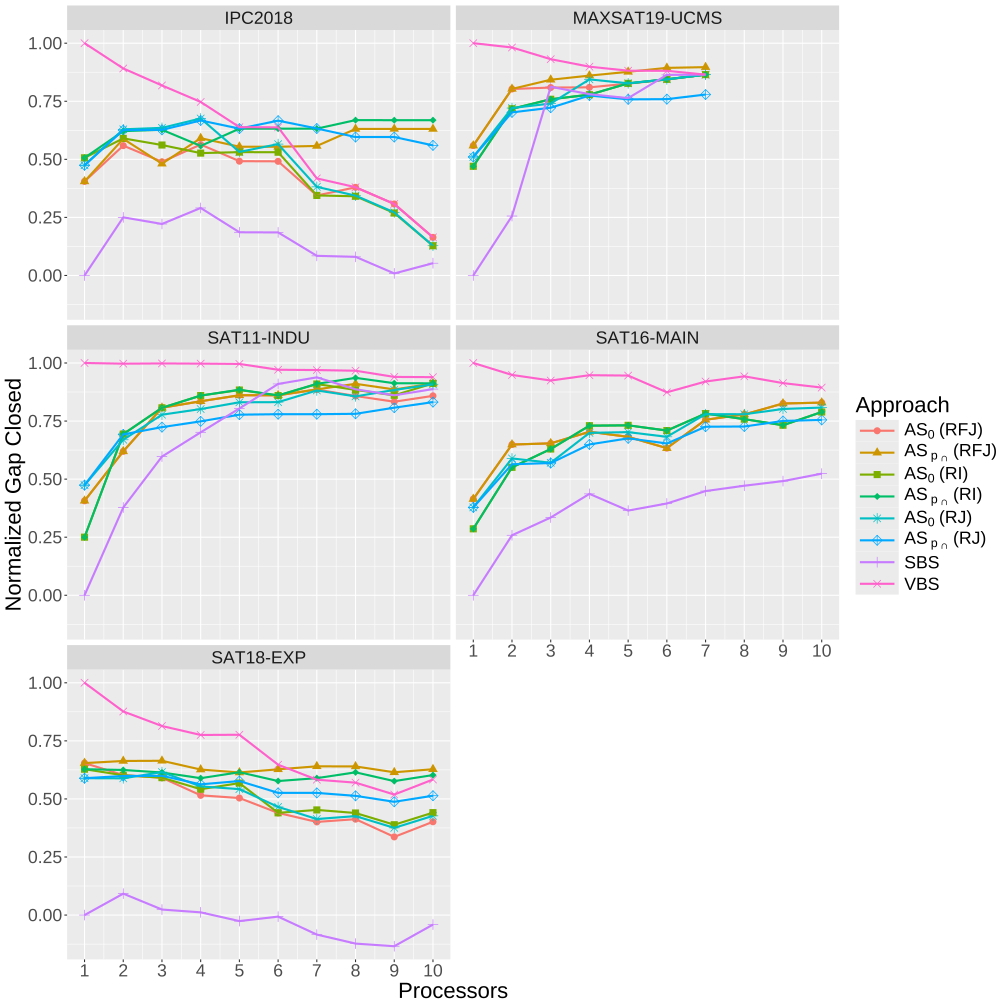
\includegraphics[width=\linewidth]{plots/learner_comparison_line_chart_parallel_NormalizedGap.pdf}    
    \caption[Results Summary: Comparing Ranger and RandomForest Models in $AS_{p_{\cap}}$ Performance]{
    Results Overview. The plot illustrates the extent to which each method narrows the gap between the PAR10 scores of the Single Best Solver (SBS) and the Virtual Best Solver (VBS). For VBS and SBS, the top $n$ solvers are selected, where $n$ matches the number of processors available for each problem instance and across all instances, respectively. $AS_0$ selects the top $n$ solvers as predicted by algorithm selection, disregarding any overlap in their predicted runtime distributions. $AS_{p_{\cap}}$ follows the approach proposed in \cite{kashgarani2023automatic}, with the number of processors capped at the specific value on the x-axis — fewer solvers than this maximum may be selected based on the overlap in runtime predictions. The RFJ model is trained with the randomForest and Jackknife method, RI uses the Ranger model with the Infinitesimal Jackknife method, and RJ applies the Ranger model with the Jackknife method. The optimal $p_{\cap}$ values for each scenario and each model are listed in Table~\ref{tab:pcap}.
    }
    \label{fig:rangervsrf}
\end{figure}

\section{Conclusions and Future Work}

In this study, we proposed a general method for selecting solvers from a portfolio of solvers and scheduling them in parallel, taking into account the predicted runtime distribution to intelligently choose not only which solvers to run, but also how many. This is in contrast to most other approaches in the literature, which either choose a constant number or use all available processors. Further, we measured the actual runtime when running more than one algorithm in parallel, rather than assuming the sequential runtime. We demonstrated substantial performance improvements across a wide range of scenarios, handily beating baseline methods and other approaches from the literature. The proposed method establishes a new state of the art in parallel algorithm selection and is simple to apply in practice -- we are only using information that is readily available in common algorithm selection methods, and while for the best performance the parameter $p_{\cap}$ of our method should be tuned, a reasonable default already shows good performance. This parameter allows our method to be tailored to specific application domains and scenarios. We also compared three different algorithm performance models, specifically three variations of the regression random forest, and applied the method to evaluate their effectiveness. 

While we do show substantial performance improvements, there is room for further advances. We have focused our investigation on state-of-the-art random forest performance models, the jackknife and infinitesimal jackknife method for estimating uncertainties. It is possible that other types of models may perform better in this context if the uncertainty estimates of their predictions are better. It is also possible to combine different types of performance models for different algorithms, allowing much more flexibility and potentially greater performance improvements. While our baseline method that allocates resources to each algorithm did not perform well, investigating more sophisticated approaches for this would also be interesting. 

Furthermore, the optimal values of $p_{\cap}$ varied significantly between different scenarios and performance models, requiring tuning for each. This can increase the complexity of the algorithm selection process, as well as the computational effort and time required for method configuration, since each scenario needs specific adjustments to achieve optimal performance. 

% Cheat to bring in other references
%\nocite{*} % delete or comment this out.
 % chapter 4
% This file is for chapter 3

\chapter{Revisiting Parallel Portfolio Selection with KL Divergence}


\section{Introduction}

Algorithms designed to solve combinatorial problems often exhibit complementary performance across different problem instances. Therefore, using a portfolio of algorithms frequently demonstrates superior performance compared to selecting the single best solver (SBS) averaged across all instances \cite{Huberman1997,GOMES200143}. Portfolios can either be run in parallel, or a single algorithm can be selected on an instance-by-instance basis by training performance models using machine learning algorithms. However, both methods have drawbacks. 

Algorithm selection has proven to be effective in solving different problems such as SAT, constraint programming, and mixed integer programming, as demonstrated by systems such as SATzilla, Hydra, and AutoFolio \cite{satzilla,lindauer2015autofolio,cphydra,XuEtAl11}. In single algorithm selection, if machine learning models are not well generalized, they might not select the correct best algorithm for a given instance. Although executing the whole portfolio of algorithms seems to avoid this issue, the more solvers that perform computations in parallel, the more time-out computations we will encounter \cite{pmlr-v140-kashgarani21a,LINDAUER2017272}. However, the proposed parallel portfolio approaches often simulate parallel execution based on sequential data, which conceals the significant overhead and performance drop that occurs when many algorithms run parallel. 

Based on the results presented in the third chapter, even with a small number of solvers, selecting a single algorithm using the imperfect regression random forest ML model can outperform parallel portfolios \cite{pmlr-v140-kashgarani21a}. In Chapter 4, we proposed a hybrid approach that leverages both algorithm selection and parallel execution. We introduced a middle-path strategy that identifies the most promising subset of algorithms to run simultaneously on a single non-distributed computer \cite{kashgarani2023automatic}. This innovative method demonstrated improved performance by utilizing three regression random forest algorithm selectors with different implementations and uncertainty estimation methods.

Using the method proposed in the previous chapter, it is possible to select an instance-based subportfolio of solvers to run in parallel, avoiding the drawbacks of algorithm selection and reducing the overhead associated with running too many solvers simultaneously. This method can achieve optimal or near-optimal performance, provided the virtual best solver is included in the selected subset of algorithms. We used the estimated uncertainty of the predictions while considering the impact of overhead from running the portfolio in parallel. 

However, this strategy still has some limitations. Specifically, the threshold value $p_{\cap}$--which is defined as the threshold for the joint probability between the prediction distributions of the minimum predicted algorithm and other algorithms, and serving as a measure of the likelihood that an algorithm is predicted to perform very closely to the minimum predicted algorithm—could not be generalized across all scenarios and algorithm performance models, as the tuned values varied significantly. Here, we aim to provide an alternative formulation for subportfolio selection that overcomes this limitation.

In this chapter, we revisit the method of selecting the optimal parallel subportfolio of algorithms to run on a single computing machine. Similar to the main proposed method, we incorporate the uncertainty of the performance predictions. Here, rather than using the threshold $p_\cap$ in Equation~\ref{eq:7} as an estimate of the probability that the algorithm is as good as the best predicted algorithm, we investigated the use of the Kullback–Leibler (KL) divergence method, which measures the difference between the probability distributions of the predicted algorithms. This method provides an understanding of the differences between algorithm predictions, in contrast to the joint probability approach, which focused on the similarity of predictions. This enables a redefined selection criterion based on the divergence from the best-predicted performance distribution.



\section{Revisit Parallel Portfolio Selection}

We aim to select a subset of solvers \begin{math} P_i \subseteq S \end{math} for a given instance \(i \in I\), prioritizing algorithms predicted to perform best (\( A \in S \) and \( A \in P_i \)) based on their predicted performance \(\hat{m}\). For each instance, a total ranking of algorithms in the portfolio \(S\) is established using their predicted performance:

\[
A < B \quad \text{if} \quad \hat{m}(A, i) < \hat{m}(B, i); A, B \in S
\]

From this ranking, the rank \(r_{A, i}\) is assigned to each algorithm \(A\), representing the number of algorithms predicted to outperform \(A\) on instance \(i\). A portfolio of size \(n\) is then defined by the top \(n\) ranked algorithms:

\[
P_i = \{A \in S \: | \: r_{A,i} \leq n\}
\]

This method allows the selection of a subset of solvers for parallel execution, balancing the likelihood of including the best-performing solver with the overhead of running multiple solvers. However, the critical challenge in parallel portfolios is determining the appropriate portfolio size $n$ for each problem instance. To address this balance, we incorporate the predicted performance distribution of algorithms and their associated uncertainty. 

Similar to the proposed method in Chapter 4, instead of considering only a point prediction, we consider the predicted distribution of performance metric values, characterized by its mean and standard deviation. Formally, we denote the standard deviation of the prediction \begin{math}\hat{m}(A, i)\end{math} as \begin{math}\sigma_{A, i}\end{math} for each solver $A$ and instance $i$. We assume that the predictions of our performance models follow a normal distribution, i.e. the predicted value is the mean of that distribution, and allow us to characterize it completely together with the standard deviation. In the previous approach, we assess the likelihood that two algorithms perform equally well by calculating the overlap area between their prediction distributions. If two algorithms are predicted to perform very similarly, then the overlap area between the distributions will be very large. Here, we replace this method by considering the Kullback–Leibler (KL) divergence between the two univariate Gaussian distributions. KL divergence captures the divergence in shape and spread between the distributions.

We are in particular interested in the predicted performance distribution of the best-predicted algorithm $A_{1,i}$ (no algorithms are predicted to perform better than it), and how the predictions for the other algorithms compare to it. Formally, for the best predicted solver $A_{1,i}$ on instance $i$ the distribution of predictions is \begin{math} \hat{m}(A_{1,i}, i) \sim \hat{M}(\mu_{A_{1,i},i}, \sigma^2_{A_{1,i},i}) \end{math} with probability density function \begin{math} f_{A_{1,i},i}\end{math} and cumulative distribution function \begin{math} F_{A_{1,i},i}\end{math}. The performance distributions for other algorithms are defined similarly.

The Kullback–Leibler (KL) divergence is a statistical metric used to quantify the difference between two probability distributions \cite{KL}. According to the formulation in \cite{bishop2006pattern}, given two distributions $p$ and $q$ with probability density functions $p(x)$ and $q(x)$, the KL divergence is calculated as:

\begin{equation}\label{eq:5.4}
    KL(p \| q) = - \int p(x) \log q(x) \, dx + \int p(x) \log p(x) \, dx
\end{equation}

In our context, we are interested in comparing the predicted performance distributions of two algorithms, $A_{x}$ and $A_{y}$, on a specific instance $i$. Let $f_{A_{x},i}$ and $f_{A_{y},i}$ denote the probability density functions of the predicted performance of algorithms $A_{x}$ and $A_{y}$ on instance $i$, respectively. By substituting $p(x)$ with $f_{A_{x},i}$ and $q(x)$ with $f_{A_{y},i}$, we adapt the KL divergence to quantify the difference in predicted performance between the two algorithms. Thus, the KL divergence between the performance distributions of $A_{x}$ and $A_{y}$ in instance $i$ is computed as follows:

\begin{equation}\label{eq:5.5} KL(f_{A_{x},i} \| f_{A_{y},i}) = - \int f_{A_{x},i}(x) \log f_{A_{y},i}(x) dx + \int f_{A_{x},i}(x) \log f_{A_{x},i}(x) dx \end{equation}

This formulation indicates to what extent the probability distributions differ. Since the two distributions are univariate Gaussians, the exact formula for KL divergence is as follows (we omit the index $i$ for the sake of brevity here):

\begin{equation}\label{eq:5.6}
    KL(f_{A_x} \| f_{A_y}) = \log \frac{\sigma_{A_y}}{\sigma_{A_x}} + \frac{\sigma_{A_x}^2 + (\mu_{A_x} - \mu_{A_y})^2}{2 \sigma_{A_y}^2} - \frac{1}{2}
\end{equation}

We define $kl \in [0, \infty)$ as a threshold for the computed KL divergence to include a given algorithm:

\begin{equation}\label{eq:5.7}
 P_i = \{A \:| \:  KL(f_{A_{1,i},i} \| f_{A_{x,i},i}) \leq \\kl\:\}
\end{equation}

$kl$ is 0 for the best predicted algorithm. In contrast to $p_{\cap}$, which could only be in the range of [0,1], the value of $kl$ can be greater than 1. A very large value of $kl$ corresponds to algorithms whose distributions diverge the most from that of the best predicted algorithm, that is, algorithms with performance predictions that are markedly different from those of the best predicted algorithm.

We can adjust the size of the parallel portfolio by modifying the $kl$ threshold. When $kl$ is set to 0, only the best predicted algorithm and those expected to perform identically are included. Setting $kl$ to a very large positive value allows all algorithms to be included. Finding the optimal $kl$ is necessary to determine how many solvers to include in the portfolio. This flexibility enables us to tailor the approach to specific algorithm selection scenarios, allowing the selection of algorithms to run in parallel and accommodating any potential inaccuracies in performance predictions.

\section{Experimental Setup}
\subsection{Data Collection}

We used the same five scenarios as in the previous chapter \cite{kashgarani2023automatic}, now included in the ASlib benchmark repository \cite{BISCHL201641}: MAXSAT19-UCMS, SAT11-INDU, SAT18-EXP, SAT16-MAIN, and IPC2018. These datasets include algorithm performance data from single and parallel runs, with parallel run measurements conducted on individual machines as described in \cite{kashgarani2023automatic}. Feature extraction was performed using the SATZilla feature extraction code for MAXSAT19-UCMS, SAT11-INDU, SAT16-MAIN, and SAT18-EXP, producing 54 features, while IPC2018 features were extracted using the code from \cite{Fawcett_Vallati_Hutter_Hoffmann_Hoos_Leyton-Brown_2014}, resulting in 305 features.

\subsection{Training}
We used the same random forest regression models from Chapter 4. The random forest regression models are trained in three ways: one using the randomForest package in R and two using the Ranger package, to predict algorithm performance on specific instances. Random forests are generally recognized for their strong performance in algorithm selection and performance prediction \cite{BISCHL201641,HUTTER201479}. Given the existence of two distinct implementations, we trained the models using both \textit{randomForest} and \textit{Ranger} implementations.

Our regression random forest models are built using the MLR package with the randomForest package as dependency, and the Ranger models are trained using the MLR3 and Ranger implementations. These models predict the runtime for each solver as the mean of the underlying distribution and estimate the standard deviation. The initial random forest model and one of the Ranger models use the Jackknife method \cite{wager2014confidence, mlr}. 
The Jackknife method estimates the standard deviation of the mean predictions in all observations used to train the random forest. This technique involves training the random forest model on $n-1$ observations, leaving one out each time to make a prediction, and repeating this for each observation. The mean prediction for each tree is calculated by averaging its predictions on the left-out data points. The Jackknife method assumes that predictions follow a normal distribution, with the standard deviation indicating the uncertainty of the overall prediction. The infinitesimal jackknife method assesses the impact of each observation by slightly down-weighting it, unlike the traditional jackknife, which removes one observation at a time.

Our setup closely follows the approach in \cite{BISCHL201641} for all three models: we excluded instance features with constant values and imputed missing feature values by using the mean of all nonmissing values for each feature. The random forest hyperparameters were tuned through random search with 250 iterations, where $ntree$ was varied from 10 to 200 and
$mtry$ from 1 to 30, using nested cross-validation with three inner folds and 10 outer folds \cite{BISCHL201641}.

\subsection{Tuning $kl$ and $p_{\cap}$}

\begin{table}
\centering
\caption{Optimum value of $kl$ for each benchmark and model.}
\label{tab:kl}
\begin{tabular}{p{3.6cm} cccc}
\toprule
Scenario & RandomForest\_Jackknife & Ranger\_Jackknife & Ranger\_Inifinitesimal\\
\midrule
IPC2018 & 0.71 & 2.35 & 2.39 \\
MAXSAT19-UCMS & 0.63 & 2.7 & 2.7\\
SAT11-INDU & 0.55 & 1.62 & 1.94\\
SAT16-MAIN & 2.66 & 2.06 & 2.96\\
SAT18-EXP & 0.12 & 1.81 & 1.35\\
\midrule
Generic best & 0.41 & 2.65 & 2.82\\
\bottomrule
\end{tabular}
\end{table}

The tuned $p_{\cap}$ value for each benchmark and each random forest model is listed in Table \ref{tab:pcap} and we are using the same values in this chapter. These values were individually optimized for each scenario to ensure that the selected portfolio provided the best balance between performance and computational efficiency. For tuning $kl$, we perform a grid search to determine the optimal value in Equation~\ref{eq:5.7} for each scenario. The search is carried out over the interval $[0, 3)$ with a resolution $0.01$, resulting in 300 possible values. 

The tuned $p_{\cap}$ value for each benchmark and each random forest model is listed in Table \ref{tab:pcap}, and we use the same values in this chapter. These values were individually optimized for each scenario to ensure that the selected portfolio provided the best balance between performance and computational efficiency. For tuning $kl$, we perform a grid search to determine the optimal value in Equation~\ref{eq:5.7} for each scenario. The search is carried out over the interval $[0, 3)$ with a resolution of 0.01, resulting in 300 possible values.

\subsection{Baselines}

For all the comparisons mentioned, we evaluate the performance of our approaches against several baseline methods. Specifically, we compare to the sequential virtual best solver (VBS), which picks the best solver for each problem instance with a cumulative misclassification penalty of zero, and to the sequential single best solver (SBS), which is the solver with the best average performance across all instances and a cumulative misclassification penalty of one. For parallel runs, the VBS is the best solver for each instance but includes the overhead for $n$ parallel runs. The parallel SBS is determined similarly, using the solvers with the best average performance instead of the best for each instance. We executed multiple solvers in parallel to capture the real run-time of the best solver in this setup, instead of assuming that it would run sequentially.

We have three algorithm selectors: RFJ (random forest with Jackknife), RJ (Ranger with Jackknife), and RI (Ranger with infinitesimal Jackknife). Each algorithm selector has five approaches for comparison. The first involves selecting algorithms on a per-instance basis, running the top $n$ predicted algorithms in parallel without accounting for any uncertainty the subportfolio selection approaches. Using the notation introduced in the previous chapter, we assign $p_{\cap}=0$ and limit the number of runs to match the available processors. Also, when we assign $kl = \infty$, we are doing the same thing and limiting the number of runs to match the available processors. The second approach uses the associated tuned $p_{\cap}$ values mentioned in Table~\ref{tab:pcap}. The third approach uses the average $p_{\cap}$ value, which was the best generic value across all scenarios. Other approach uses the associated tuned $kl$ values mentioned in Table~\ref{tab:kl} for each scenario and performance model. The last approach uses the generic best $kl$ value across all scenarios for each performance model.

We evaluate the proposed method by measuring the penalized average runtime with a factor of 10 (PAR10), the misclassification penalty (MCP), and the runtime. The PAR10 metric equals the actual runtime if the algorithm successfully solves the instance within the timeout; otherwise, it is calculated as the timeout multiplied by 10. The MCP represents the difference between the performance of the selected algorithm and that of the optimal algorithm. The mean and standard deviation of these values are presented in Tables~\ref{tab:summary5-ipc-max},\ref{tab:summary5-sat11-sat16}, and\ref{tab:summary5-sat18}. We normalize PAR10 values across scenarios using the performances of the VBS and SBS, reporting the proportion of the performance gap each approach bridges. On this normalized scale, 0 denotes the performance of the SBS, while 1 denotes the performance of the VBS. 

In the tables, we report the mean and standard deviation of the normalized gap closed across the 10 folds of data used to train the performance models. In contrast to the reported runtime, MCP, and PAR10 scores, where we present the mean and standard deviation across the distribution of all instances. We use folds here to avoid zero denominators in cases where the single best solver is the actual best solver for an instance, based on the normalized gap closed formula $\frac{\text{sbs} - \text{approach}}{\text{sbs} - \text{vbs}}$. The plots~\ref{fig:all_results}, show the PAR10 score normalized gap closed over the entire distribution of instances.

\section{Results}
\subsection{Tuning of $kl$ and $p_{\cap}$}

Tuning $p_{\cap}$ and $kl$ reveals that the optimal values vary by scenario. Tables~\ref{tab:pcap} and~\ref{tab:kl} present the optimal values for each scenario and algorithm selector. We presented Figure~\ref{fig:kl_sensitivity}, which shows the normalized gap closed for the mean, 25th percentile, 50th percentile, and 75th percentile across each scenario based on $kl$ value. Although optimal values vary significantly between scenarios and performance models, normalized gaps closed remain relatively small as long as $kl$ is not too low. For the most optimal performance, we recommend tuning $kl$ for each specific scenario.

The optimal value of $kl$, similar to $p_{\cap}$, provides insight into the predictive accuracy of the performance models. A large $kl$ value suggests that the models' predictions may lack accuracy, as it requires including solvers whose predicted runtime distributions differ significantly from that of the best predicted solver in order to capture solvers that perform well. If the optimal value of $kl$ were 0, we would include only solvers that are exactly similar to the best-predicted solver. A very large optimal $kl$ requires us to include all solvers, even those whose predicted distributions differ entirely from the best predicted solver. 

Here, the optimal values for $kl$ are relatively small, typically up to 2.5 in most cases. The further the $kl$ value deviates from 0, the lower the accuracy. Table~\ref{tab:kl} also shows that the RFJ model, which uses randomForest with a Jackknife uncertainty estimate, has a significantly lower optimal $kl$ in most scenarios, suggesting that this model should outperform the other two when selecting single solver in 4 out of 5 scenarios in terms of prediction accuracy. This is confirmed by Tables~\ref{tab:summary5-ipc-max}, \ref{tab:summary5-sat11-sat16} and~\ref{tab:summary5-sat18} which is denoted as $AS (RFJ)$. The optimal $kl$ values are closer for all scenarios when we have a single model. This seems to contrast with $p_{\cap}$, where different scenarios had significantly varying values per model. Here, the values are more consistent, suggesting that tuning this parameter per model should yield good performance.

\subsection{$AS_{p_{\cap}}$ vs. $AS_{kl}$ Comparison}

To evaluate the effectiveness of any of the approaches, we carried out a series of experiments using the optimum best value for $p_{\cap}$ and $kl$ and $p_{\cap} = 0$ for each scenario, where we varied the number of processors used for parallel execution from one to ten for the scenarios SAT18-EXP, SAT16-MAIN, SAT11-INDU and IPC2018. For the MAXSAT19-UCMS scenario, we used a maximum of seven processors, as there are only seven algorithms. Figure~\ref{fig:klvspcap} shows the PAR10 score results in terms of the normalized performance gap closed between the sequential single best solver and the sequential virtual best solver for all scenarios and number of processors. In addition, Tables~\ref{tab:summary5-ipc-max},~\ref{tab:summary5-sat11-sat16} and~\ref{tab:summary5-sat18} show the mean and standard deviation values for runtime, MCP and PAR10 when limiting the maximum number of parallel runs to 10 or SAT18-EXP, SAT16-MAIN, SAT11-INDU and IPC2018, and to 7 for MAXSAT19-UCMS. In addition, we reported the mean and standard deviation of the normalized gap closed across folds in these tables. This differs from the plots, as the plots report values in terms of the mean of the problem distribution rather than across folds.

Here, we discuss the results of the comparison of $AS_{p_{\cap}}$ with the $AS_{kl}$ methods. For this comparison, we excluded the results of the RJ model in Figure~\ref{fig:klvspcap} because, as mentioned in the previous section comparing ranger and randomForest, the RJ model did not outperform the other two models in subportfolio selection, while RI and RFJ were competitive in portfolio selection. This is also evident in Tables~\ref{tab:summary5-ipc-max}, \ref{tab:summary5-sat11-sat16}, and~\ref{tab:summary5-sat18} that the RJ model did not surpass the other two when using $AS_{p_{\cap}}$ and $AS_{kl}$. Therefore, we discuss the results for the RI and RFJ models when selecting subportfolios using Equation~\ref{eq:7}, denoted as $AS_{p_{\cap}}$, and Equation~\ref{eq:5.7}, denoted as $AS_{kl}$.

When comparing $AS_{p_{\cap}}$ and $AS_{kl}$ with optimal threshold values, based on Tables~\ref{tab:summary5-ipc-max}, \ref{tab:summary5-sat11-sat16}, and~\ref{tab:summary5-sat18}, $AS_{kl}$ outperforms $AS_{p_{\cap}}$ in three of four performance metrics for IPC2018 and the RFJ model. For the RI model, $AS_{p_{\cap}}$ is superior in three of the four metrics, while for the RJ model, $AS_{kl}$ performs worse in all performance metrics. Figure~\ref{fig:klvspcap} further illustrates that $AS_{p_{\cap}}$ consistently outperforms $AS_{kl}$ for both the RFJ and RI models when the cores are limited to different values. For the MAXSAT19-UCMS and SAT11-INDU scenarios, $AS_{p_{\cap}}$ performs better than $AS_{kl}$ in all performance metrics for the RJ, RFJ, and RI models, which is also reflected in the closed mean normalized gap in Figure~\ref{fig:klvspcap}. In the SAT16-MAIN scenario, $AS_{p_{\cap}}$ is overall superior, except for the RFJ model, where both methods perform equally, and the RJ model where the normalized gap closed for folds is slightly worse for $AS_{p_{\cap}}$. In the SAT18-EXP scenario, $AS_{p_{\cap}}$ generally outperforms $AS_{kl}$, except for the RFJ model where the two are highly competitive. In three of four performance metrics, $AS_{kl}$ is better, while $AS_{p_{\cap}}$ excels in the remaining metric.

When comparing the RFJ and RI models for portfolio selection using the $AS_{kl}$ method, the RFJ model performed consistently best in all scenarios. This contrasts with the $AS_{p_{\cap}}$ approach, where the RI model outperformed the RFJ model in two out of five scenarios. When comparing $AS_{p_{\cap}}$ and $AS_{kl}$ using the generic best values across the tuned scenarios for each model, $AS_{p_{\cap}}$ outperforms $AS_{kl}$ in two of the three models for IPC2018, MAXSAT19-UCMS and SAT16-MAIN. However, for the RFJ model in these scenarios, the trend is reversed, with $AS_{kl}$ performing slightly worse. For SAT11-INDU and SAT18-EXP, $AS_{p_{\cap}}$ is the consistently better approach across all models.

When comparing all the experimented methods in all scenarios with the number of parallel runs limited to 10, the $AS_{p_{\cap}}$ of the RI model delivered the best performance for IPC2018 and SAT11-INDU in terms of runtime, MCP, normalized gap, and PAR10. For these scenarios, $AS_{kl}$ of the RI model was the second-best method. For MAXSAT19-UCMS, the $AS_{p_{\cap}}$ of the RFJ model achieved the best performance, followed by the $AS_{kl}$ of the RFJ model as the second-best method. In SAT16-MAIN, $AS_{p_{\cap}}$ of the RI model, with $p_{\cap}$ set to zero and selecting the top 10 predicted algorithms, emerged as the best method. The second-best method in this scenario was the $AS_{p_{\cap}}$ of the RI model, using the generic best value for $p_{\cap}$. Finally, for SAT18-EXP, the $AS_{p_{\cap}}$ and $AS_{kl}$ methods of the RFJ model performed very competitively, both achieving the best performance. 

Although the $AS_{p_\cap}$ method appears to be in general superior to $AS_{kl}$, its performance is very close, making $AS_{kl}$ the best alternative in the absence of $AS_{p_\cap}$. One significant advantage of $AS_{kl}$ is that the tuned values of $kl$ for different scenarios are highly consistent, and this suggests that tuning of $kl$ globally across all scenarios can still produce good performance. This consistency reduces the cost of scenario-specific tuning. In contrast, the $p_{\cap}$ values vary significantly between different models, and it makes tuning more challenging and model-dependent. On the other hand, $kl$ demonstrates greater consistency, with its best generic values for the RI and RJ models being close, which further highlights its practicality for streamlined optimization.

\begin{figure}
\centering
    \includegraphics[width=0.49\linewidth]{plots/kl_div_rfj_sensitivity_x_theta_y_runtime_facet.pdf}
    \includegraphics[width=0.49\linewidth]{plots/kl_ri_div_sensitivity_x_theta_y_runtime_facet.pdf}
    \includegraphics[width=0.49\linewidth]{plots/kl_div_rj_sensitivity_x_theta_y_runtime_facet.pdf}
    \caption[Sensitivity of Portfolio Performance to $kl$]{Sensitivity of Portfolio Performance to $kl$. The top left plot corresponds to the RFJ model, and the top right plot corresponds to the RI model, and the bottom plot is for RJ model. The plot displays the mean, first quartile (Q1, 25th percentile), median (Q2, 50th percentile), and third quartile (Q3, 75th percentile) runtime performance for each scenario across different $kl$ values, as defined in Equation~\ref{eq:5.7}. The y-axis uses a log scale to represent the normalized gap closed, highlighting variations in performance sensitivity relative to $kl$ adjustments.}
    \label{fig:kl_sensitivity}
\end{figure}

\begin{figure}
        \includegraphics[width=\linewidth]{plots/kl_pcap_comparison_line_chart_parallel_NormalizedGap.pdf}    
    \caption[Results Summary: Comparing $AS_{p_{\cap}}$ with $AS_{kl}$ Performance]{
    Results Overview. The plot illustrates the extent to which each method narrows the gap between the PAR10 scores of the Single Best Solver (SBS) and the Virtual Best Solver (VBS). For VBS and SBS, the top $n$ solvers are selected, where $n$ matches the number of processors available for each problem instance and across all instances, respectively. $AS_{p_{\cap}}$ and $AS_{kl}$ follow the approaches proposed in \cite{kashgarani2023automatic} and Equation~\ref{eq:5.7}, respectively, with the number of processors capped at the specific value on the x-axis — fewer solvers than this maximum may be selected based on the overlap and divergence in runtime predictions. The RFJ model is trained with the randomForest and Jackknife method, RI uses the Ranger model with the Infinitesimal Jackknife method. The optimal $p_{\cap}$ and $kl$ values for each scenario and each model are listed in Tables~\ref{tab:pcap} and~\ref{tab:kl}.
    }
    \label{fig:klvspcap}
\end{figure}

\begin{table}
\begin{center}
    {\caption[Detailed Results: Runtime, MCP, PAR10, and Normalized Gap Closed for $AS_{p_{\cap}}$ vs. $AS_{kl}$ for IPC2018 and MAXSAT19-UCMS Scenarios]{Detailed results. Mean and standard deviation of values for runtime, MCP, and PAR10 across all problem instances in a scenario for the sequential virtual best solver, sequential single best solver, and single top predicted algorithm in the initial three rows. The second set of rows for each scenario shows the results for the maximum number of processors (10 for IPC2018, and 7 for MAXSAT19-UCMS) for our approaches and the baselines we compare to. All numbers were rounded to integers. The best value for each scenario and measure is shown in \textbf{bold} (excepting the sequential VBS, which is by definition always the best), the second best in \textit{italics}. The normalized gap closed represents the mean and standard deviation of the normalized gap closed across the folds.}\label{tab:summary5-ipc-max}}
    \scriptsize\begin{tabular}{clcccc}
    \toprule
        Scenario & Approach & Runtime [s] & MCP & PAR10 & NormalizedGap\\
    \midrule
    
    \multirow{20}{*}{\rotatebox{90}{IPC2018}} & \multicolumn{5}{c}{\textbf{1 Processor}} \\\cmidrule{2-6}        
        & VBS & 508$\pm$697 & 0 & 3478$\pm$6903 & 1\\
        & AS (RFJ) & 607$\pm$751 & 99$\pm$301 & 4657$\pm$7725 & -0.44$\pm$2.84\\
        & AS (RI) & 608$\pm$751 & 100$\pm$293 & 4456$\pm$7583 & -0.35$\pm$2.85\\
        & AS (RJ) & 604$\pm$752 & 96$\pm$293 & 4519$\pm$7633 & -0.39$\pm$2.84 \\
        & SBS & 734$\pm$770 & 226$\pm$414 & 5459$\pm$8072 & 0 \\
    \cmidrule{2-6}  
    & \multicolumn{5}{c}{\textbf{10 Processors}}\\
    \cmidrule{2-6}
        %& VBS &  &  &  \\
        %& SBS &  &  & \\
        & $AS_{p_{\cap} = 0}$ (RFJ) & 612$\pm$779 & 104$\pm$307 & 5134$\pm$8027 & -0.66$\pm$2.56\\
        & $AS_{p_{\cap} = 0}$ (RI)  & 616$\pm$783  & 107$\pm$312 & 5206$\pm$8065 & -0.69$\pm$2.54\\
        & $AS_{p_{\cap} = 0}$ (RJ)  & 616$\pm$783 & 107$\pm$312 & 5206$\pm$8065 & -0.69$\pm$2.54 \\ 
        & $AS_{p_{\cap} = 0.59}$ (RFJ) & 569$\pm$745 & 61$\pm$223 & 4484$\pm$7651 & \textbf{-0.18$\pm$2.74} \\
        & $AS_{p_{\cap} = 0.44}$ (RI) & \textbf{557$\pm$728} & \textbf{49$\pm$190} & \textbf{4135$\pm$7403} & \emph{-0.19$\pm$2.89}\\
        & $AS_{p_{\cap} = 0.27}$ (RJ) & 570$\pm$744 & 62$\pm$229 & 4350$\pm$7552 &  -0.21$\pm$2.72 \\
        & $AS_{p_{\cap} = 0.82}$ (RFJ) & 579$\pm$742 & 70$\pm$233 & 4359$\pm$7548  & -0.26$\pm$2.88 \\
        & $AS_{p_{\cap} = 0.17}$ (RI) & 570$\pm$739 & 62$\pm$230 & 4283$\pm$7501 & -0.24$\pm$2.87\\
        & $AS_{p_{\cap} = 0.31}$ (RJ) & 570$\pm$743 & 62$\pm$229 & 4350$\pm$7552 & -0.21$\pm$2.72\\
        & $AS_{kl = 0.71} (RFJ)$ & \emph{560$\pm$735} & \emph{52$\pm$193} & \emph{4272$\pm$7506} & -0.19$\pm$2.71\\
        & $AS_{kl = 2.39} (RI)$ & 570$\pm$740 & 62$\pm$224 & 4350$\pm$7552 & -0.3$\pm$2.86\\
        & $AS_{kl = 2.35} (RJ)$ & 577$\pm$750 & 70$\pm$243 & 4492$\pm$7647 & -0.31$\pm$2.67 \\ 
        & $AS_{kl = 0.41} (RFJ)$ & 571$\pm$738 & 63$\pm$220 & 4351$\pm$7551 & -0.23$\pm$2.73\\ 
        & $AS_{kl = 2.82} (RI)$ & 575$\pm$746 & 67$\pm$244 & 4423$\pm$7599 & -0.32$\pm$2.85\\ 
        & $AS_{kl = 2.65} (RJ)$ & 577$\pm$750 & 70$\pm$243 & 4492$\pm$7647 & -0.31$\pm$2.67 \\
        
    \midrule
    \multirow{22}{*}{\rotatebox{90}{MAXSAT19-UCMS}} & \multicolumn{5}{c}{\textbf{1 Processor}} \\\cmidrule{2-6}
        & VBS & 858$\pm$1476 & 0 & 7768$\pm$14717 & 1\\
        & AS (RFJ) & 1037$\pm$1555 & 179$\pm$641 & 9363$\pm$15684 & 0.55$\pm$0.28\\
        & AS (RI) & 1076$\pm$1575 & 218$\pm$729 & 9686$\pm$15850 & 0.45$\pm$0.34 \\
        & AS (RJ) & 1044$\pm$1565 & 186$\pm$666 & 9540$\pm$15793 & 0.49$\pm$0.23 \\
        & SBS & 1190$\pm$1657 & 332$\pm$940 & 11386$\pm$16696 & 0 \\
    \cmidrule{2-6}   
    & \multicolumn{5}{c}{\textbf{7 Processors}}\\
    \cmidrule{2-6}  
        & $AS_{p_{\cap} = 0}$ (RFJ) & 894$\pm$1506 & 37$\pm$247 & 8258$\pm$15062 & 0.85$\pm$0.16\\
        & $AS_{p_{\cap} = 0}$ (RI) & 894$\pm$1506 & 37$\pm$247 & 8258$\pm$15062 & 0.85$\pm$0.16 \\ 
        & $AS_{p_{\cap} = 0}$ (RJ) & 894$\pm$1506 & 37$\pm$247 & 8258$\pm$15062 & 0.85$\pm$0.16\\
        & $AS_{p_{\cap} = {0.55}}$ (RFJ) & \textbf{891$\pm$1496} & \textbf{33$\pm$215} & \textbf{8141$\pm$14975} & \textbf{0.88$\pm$0.17} \\
        & $AS_{p_{\cap} = 0.03}$ (RI) & 894$\pm$1506 & 37$\pm$247 & 8258$\pm$15062 & 0.85$\pm$0.16  \\ 
        & $AS_{p_{\cap} = 0.14}$ (RJ) & 921$\pm$1521 & 63$\pm$369 & 8568$\pm$15263 &  0.76$\pm$0.24 \\
        & $AS_{p_{\cap} = 0.82}$ (RFJ) & 928$\pm$1513 & 70$\pm$364 & 8461$\pm$15175 & 0.81$\pm$0.18\\
        & $AS_{p_{\cap} = 0.17}$ (RI) & 901$\pm$1502 & 43$\pm$275 & 8208$\pm$15015 &  \emph{0.88$\pm$0.16} \\
        & $AS_{p_{\cap} = 0.31}$ (RJ) & 931$\pm$1525 & 73$\pm$402 & 8578$\pm$15259 & 0.78$\pm$0.21 \\
        & $AS_{kl = 0.63} (RFJ)$ & \emph{892$\pm$1495} & \emph{35$\pm$216} & \emph{8143$\pm$14974} & \textbf{0.88$\pm$0.17} \\
        & $AS_{kl = 2.7} (RI)$ & 920$\pm$1517 & 63$\pm$349 & 8454$\pm$15179 & 0.82$\pm$0.17\\ 
        & $AS_{kl = 2.7} (RJ)$ & 931$\pm$1530 & 74$\pm$409 & 8691$\pm$15342 & 0.74$\pm$0.25\\
        & $AS_{kl = 0.41} (RFJ)$ & 915$\pm$1513 & 57$\pm$335 & 8448$\pm$15182 & 0.8$\pm$0.19\\ 
        & $AS_{kl = 2.82} (RI)$ & 921$\pm$1517 & 63$\pm$349 & 8454$\pm$15179 & 0.82$\pm$0.17\\ 
        & $AS_{kl = 2.65} (RJ)$ & 931$\pm$1530 & 74$\pm$409  & 8691$\pm$15342 & 0.74$\pm$0.25 \\
  
    \bottomrule
    \end{tabular}    
\end{center}
\end{table}

\begin{table}
\begin{center}
    {\caption[Detailed Results: Runtime, MCP, PAR10, and Normalized Gap Closed for $AS_{p_{\cap}}$ vs. $AS_{kl}$ for SAT11-INDU and SAT16-MAIN Scenarios]{Detailed results. Mean and standard deviation of values for runtime, MCP, and PAR10 across all problem instances in a scenario for the sequential virtual best solver, sequential single best solver, and single top predicted algorithm in the initial three rows. The second set of rows for each scenario shows the results for the maximum number of processors (10 for SAT16-MAIN and SAT11-INDU) for our approaches and the baselines we compare to. All numbers were rounded to integers. The best value for each scenario and measure is shown in \textbf{bold} (excepting the sequential VBS, which is by definition always the best), the second best in \textit{italics}. The normalized gap closed represents the mean and standard deviation of the normalized gap closed across the folds.}\label{tab:summary5-sat11-sat16}}
    \scriptsize\begin{tabular}{clcccc}
    \toprule
        Scenario & Approach & Runtime [s] & MCP & PAR10 & NormalizedGap\\
    \midrule
    \multirow{23}{*}{\rotatebox{90}{SAT11-INDU}} & \multicolumn{5}{c}{\textbf{1 Processor}} \\\cmidrule{2-6}
        & VBS & 1140$\pm$1836 & 0 & 8040$\pm$17905 & 1\\
        & AS (RFJ) & 1535$\pm$2058 & 395$\pm$1037 & 11735$\pm$20768 & 0.16$\pm$0.79\\        
        & AS (RI) & 1610$\pm$2108 & 470$\pm$1145 & 12710$\pm$21389 & -0.06$\pm$0.9\\
        & AS (RJ) & 1565$\pm$2049 & 425$\pm$1017 & 11315$\pm$20402 & 0.34$\pm$0.49\\
        & SBS & 1818$\pm$2168 & 678$\pm$1340 & 14268$\pm$22154 & 0 \\
    \cmidrule{2-6}    
    & \multicolumn{5}{c}{\textbf{10 Processors}}\\
    \cmidrule{2-6}    
        & $AS_{p_{\cap} = 0}$ (RFJ) & 1272$\pm$1927 & 161$\pm$548 & 8922$\pm$18645 & \emph{0.89$\pm$0.12}\\
        & $AS_{p_{\cap} = 0}$ (RI) & \emph{1238$\pm$1892} & 127$\pm$385 & \emph{8588$\pm$18350} & \textbf{0.92$\pm$0.1}\\ 
        & $AS_{p_{\cap} = 0}$ (RJ) & 1262$\pm$1910 & 151$\pm$480 & 8612$\pm$18342 & \textbf{0.92$\pm$0.1} \\
        & $AS_{p_{\cap} = 0.63}$ (RFJ) & 1241$\pm$1901 & 131$\pm$451 & 8591$\pm$18349 & \textbf{0.92$\pm$0.1} \\
        & $AS_{p_{\cap} = 0.01}$ (RI) & \textbf{1236$\pm$1890} & \textbf{121$\pm$379} & \textbf{8586$\pm$18351} & \textbf{0.92$\pm$0.1} \\ 
        & $AS_{p_{\cap} = 0.31}$ (RJ) & 1289$\pm$1934 & 178$\pm$595 & 9089$\pm$18787 & 0.78$\pm$0.28\\
        & $AS_{p_{\cap} = 0.82}$ (RFJ) & 1247$\pm$1900 & \emph{123$\pm$431} & 8747$\pm$18501 &  0.83$\pm$0.28 \\
        & $AS_{p_{\cap} = 0.17}$ (RI) & 1259$\pm$1912 & 139$\pm$477 & 8909$\pm$18649 & 0.74$\pm$0.36\\
        & $AS_{p_{\cap} = 0.31}$ (RJ) & 1289$\pm$1934 & 178$\pm$595 & 9089$\pm$18787 & 0.78$\pm$0.28 \\
        & $AS_{kl = 0.55} (RFJ)$ & 1243$\pm$1902 & 132$\pm$450 & 8593$\pm$18349 & \textbf{0.92$\pm$0.1} \\
        & $AS_{kl = 1.62} (RI)$ & 1283$\pm$1931 & 158$\pm$539 & 9233$\pm$18936 &  0.68$\pm$0.34 \\ 
        & $AS_{kl = 1.94} (RJ)$ & 1307$\pm$1950 & 194$\pm$622 & 9407$\pm$19072 & 0.73$\pm$0.26\\
        & $AS_{kl = 0.41} (RFJ)$ & 1250$\pm$1910 & 137$\pm$465 & 8750$\pm$18501 & \emph{0.89$\pm$0.12}\\ 
        & $AS_{kl = 2.82} (RI)$ & 1288$\pm$1939 & 166$\pm$550 & 9238$\pm$18934 &  0.68$\pm$0.34 \\ 
        & $AS_{kl = 2.65} (RJ)$ & 1310$\pm$1953 & 198$\pm$626 & 9410$\pm$19071 & 0.73$\pm$0.26\\
  
   \midrule
    \multirow{25}{*}{\rotatebox{90}{SAT16-MAIN}} & \multicolumn{5}{c}{\textbf{1 Processor}} \\\cmidrule{2-6}
        & VBS & 1867$\pm$2193 & 0 & 15005$\pm$22530 & 1\\
        & AS (RFJ) & 2315$\pm$2273 & 448$\pm$1109 & 19066$\pm$23883 & 0.33$\pm$0.56\\
        & AS (RI) & 2383$\pm$2294 & 516$\pm$1151 & 19956$\pm$24111 & 0.05$\pm$0.66\\ 
        & AS (RJ) & 2400$\pm$2269 & 533$\pm$1177 & 19316$\pm$23880 & 0.3$\pm$0.24\\ 
        & SBS & 2560$\pm$2294 & 693$\pm$1415 & 21940$\pm$24464 & 0\\
    \cmidrule{2-6}
    & \multicolumn{5}{c}{\textbf{10 Processors}}\\
    \cmidrule{2-6}
        & $AS_{p_{\cap} = 0}$ (RFJ) & 2065$\pm$2221 & 198$\pm$652 & \textbf{16189$\pm$22931} & \emph{0.7$\pm$0.39}\\
        & $AS_{p_{\cap} = 0}$ (RI)& \textbf{2016$\pm$2225} & \textbf{150$\pm$503} & 16469$\pm$23122 & 0.68$\pm$0.6\\ 
        & $AS_{p_{\cap} = 0}$ (RJ)& 2048$\pm$2228 & 181$\pm$597 & 16336$\pm$23023 & 0.68$\pm$0.59\\ 
        & $AS_{p_{\cap} = 0.33}$ (RFJ) & 2065$\pm$2221 & 198$\pm$652 & \textbf{16189$\pm$22931} & \emph{0.7$\pm$0.39}\\
        & $AS_{p_{\cap} = 0}$ (RI) & \textbf{2016$\pm$2225} & \textbf{150$\pm$503} & 16469$\pm$23122 & 0.68$\pm$0.6\\ 
        & $AS_{p_{\cap} = 0.33}$ (RJ) & 2088$\pm$2239 & 222$\pm$704  & 16705$\pm$23156 & 0.64$\pm$0.37\\
        & $AS_{p_{\cap} = 0.82}$ (RFJ) & 2094$\pm$2222 & 228$\pm$730 & 16383$\pm$22993 & 0.69$\pm$0.41\\
        & $AS_{p_{\cap} = 0.17}$ (RI) & \emph{2041$\pm$2230} & \emph{174$\pm$591} & 16822$\pm$23261 & 0.57$\pm$0.63\\
        & $AS_{p_{\cap} = 0.31}$ (RJ) & 2096$\pm$2240 & 229$\pm$713 & 16877$\pm$23227 & 0.63$\pm$0.36\\   
        & $AS_{kl = 2.66} (RFJ)$ & 2065$\pm$2221 & 198$\pm$652 & \textbf{16189$\pm$22931} & \emph{0.7$\pm$0.39} \\ 
        & $AS_{kl = 2.96} (RI)$ & 2070$\pm$2236 & 204$\pm$647 & 17016$\pm$23318 & 0.64$\pm$0.59 \\ 
        & $AS_{kl = 2.06} (RJ)$ & 2104$\pm$2245 & 237$\pm$736 & 17049$\pm$23297 & 0.69$\pm$0.35\\
        & $AS_{kl = 0.41} (RFJ)$ & 2089$\pm$2223 & 223$\pm$698 & \emph{16213$\pm$22916}& \textbf{0.71$\pm$0.4} \\ 
        & $AS_{kl = 2.82} (RI)$ & 2093$\pm$2238 & 227$\pm$704 & 17203$\pm$23376 & 0.59$\pm$0.39 \\ 
        & $AS_{kl = 2.65} (RJ)$ & 2104$\pm$2245 & 237$\pm$735 & 17049$\pm$23297 & 0.62$\pm$0.36\\
\bottomrule
    
    \end{tabular}    
\end{center}
\end{table}

\begin{table}
\begin{center}
    {\caption[Detailed Results: Runtime, MCP, PAR10, and Normalized Gap Closed for $AS_{p_{\cap}}$ vs. $AS_{kl}$ for SAT18-EXP Scenario]{Detailed results. Mean and standard deviation of values for runtime, MCP, and PAR10 across all problem instances in a scenario for the sequential virtual best solver, sequential single best solver, and single top predicted algorithm in the initial three rows. The second set of rows for each scenario shows the results for the maximum number of processors (10 for SAT18-EXP) for our approaches and the baselines we compare to. All numbers were rounded to integers. The best value for each scenario and measure is shown in \textbf{bold} (excepting the sequential VBS, which is by definition always the best), the second best in \textit{italics}. The normalized gap closed represents the mean and standard deviation of the normalized gap closed across the folds.}\label{tab:summary5-sat18}}
    \scriptsize\begin{tabular}{clcccc}
    \toprule
        Scenario & Approach & Runtime [s] & MCP & PAR10 & NormalizedGap\\
    \midrule
    
    \multirow{23}{*}{\rotatebox{90}{SAT18-EXP }} & \multicolumn{5}{c}{\textbf{1 Processor}} \\\cmidrule{2-6}
         & VBS & 1146$\pm$1945 & 0 & 9687$\pm$19547 & 1\\
         & AS (RFJ) & 1615$\pm$2138 & 468$\pm$1192 & 13470$\pm$21889 & 0.64$\pm$0.18\\
         & AS (RI) & 1648$\pm$2151 & 502$\pm$1256 & 13758$\pm$22034 & 0.59$\pm$0.18\\
         & AS (RJ) & 1690$\pm$2170 & 543$\pm$1302 & 14183$\pm$22247 & 0.57$\pm$0.16\\
         & SBS & 2400$\pm$2249 & 1254$\pm$1832 & 20629$\pm$24280 & 0\\
    \cmidrule{2-6}    
    & \multicolumn{5}{c}{\textbf{10 Processors}}\\
    \cmidrule{2-6}           
         & $AS_{p_{\cap} = 0}$ (RFJ) & 1702$\pm$2301 & 559$\pm$1389 & 16235$\pm$23355 & 0.39$\pm$0.27\\
         & $AS_{p_{\cap} = 0}$ (RI) & 1654$\pm$2285 & 511$\pm$1324 & 15804$\pm$23194 & 0.42$\pm$0.29\\
         & $AS_{p_{\cap} = 0}$ (RJ) & 1678$\pm$2288 & 535$\pm$1351 & 15956$\pm$23243 & 0.4$\pm$0.3 \\
         & $AS_{p_{\cap} = 0.81}$ (RFJ) & \emph{1518$\pm$2172} & \textbf{372$\pm$1124} & \emph{13884$\pm$22265} & \emph{0.62$\pm$0.22} \\
         & $AS_{p_{\cap} = 0.55}$ (RI) & 1541$\pm$2191 & 397$\pm$1177 & 14034$\pm$22332 & \emph{0.6$\pm$0.21}\\ 
         & $AS_{p_{\cap} = 0.58}$ (RJ) & 1622$\pm$2237 & 477$\pm$1268 & 15008$\pm$22805 & 0.5$\pm$0.25\\
         & $AS_{p_{\cap} = 0.82}$ (RFJ) & 1532$\pm$2178 & 386$\pm$1146 &  14025$\pm$22336 & 0.6$\pm$0.23\\
         & $AS_{p_{\cap} = 0.17}$ (RI) & 1555$\pm$2221 & 410$\pm$1191 & 14558$\pm$22628 & 0.57$\pm$0.23\\
         & $AS_{p_{\cap} = 0.31}$ (RJ) & 1649$\pm$2265 & 505$\pm$1319 & 15544$\pm$23064 & 0.46$\pm$0.26\\
         & $AS_{kl = 0.12} (RFJ)$ & \textbf{1518$\pm$2169} & \emph{373$\pm$1129} & \textbf{13756$\pm$22187} & \textbf{0.62$\pm$0.23} \\ 
         & $AS_{kl = 1.81} (RI)$ & 1567$\pm$2213 & 422$\pm$1211 & 14442$\pm$22547 & 0.58$\pm$0.23 \\ 
         & $AS_{kl = 1.35} (RJ)$ & 1656$\pm$2268 & 512$\pm$1316 & 15551$\pm$23060 & 0.45$\pm$0.23\\
         & $AS_{kl = 0.41} (RFJ)$ & 1585$\pm$2230 & 440$\pm$1236 & 14843$\pm$22755 & 0.53$\pm$0.28\\ 
         & $AS_{kl = 2.82} (RI)$ & 1569$\pm$2227 & 424$\pm$1219 & 14699$\pm$22693 & 0.55$\pm$0.22\\ 
         & $AS_{kl = 2.65} (RJ)$ & 1669$\pm$2274 & 525$\pm$1335 & 15691$\pm$23119 & 0.43$\pm$0.22\\
  
    \bottomrule
    
    \end{tabular}    
\end{center}
\end{table}

\begin{figure}
    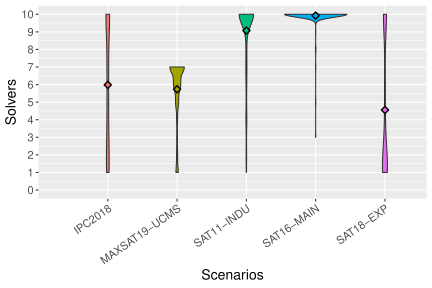
\includegraphics[width=0.5\linewidth]{plots/number_of_solvers_rf_kl.pdf}
    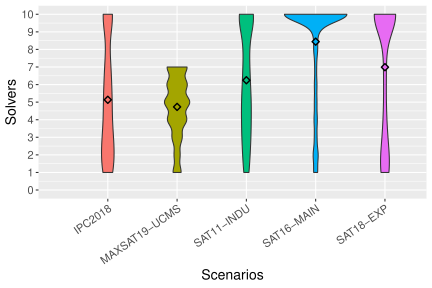
\includegraphics[width=0.5\linewidth]{plots/number_of_solvers_infjack_kl.pdf}
    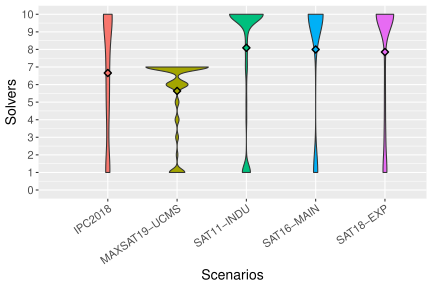
\includegraphics[width=0.5\linewidth]{plots/number_of_solvers_jack_kl.pdf}

    \caption[Distribution of Number of Selected Solvers when Using $AS_{kl}$]{
    Violin plot of the distribution of the number of selected solvers to run in parallel across all problem instances for each scenario for the respective optimal $kl$ and the maximum level of parallelism (seven processors for MAXSAT19-UCMS and 10 for all other scenarios). The diamond denotes the mean value. The top-left plot refers to the RFJ model, the top-right plot to the RI model, and the bottom plot to the RJ model.
    }
    \label{fig:numberofsolvers_kl}
\end{figure}


\section{Conclusions and Future Work}

In this study, we proposed a variation of the method introduced in Chapter 4 and expanded our experiments to incorporate these adaptations. We developed an alternative general approach for selecting solvers from a portfolio and scheduling them in parallel. This method leverages the predicted runtime distribution to make informed decisions about which solvers and how many to run in parallel. Specifically, in contrast to the method introduced in Chapter 4, where the joint probability of the prediction distribution is used as a measure of the likelihood that an algorithm performs, as well as the best-predicted solver, the new approach utilizes the KL divergence formula. This allows us to evaluate how much an algorithm's prediction diverges from the best-predicted solver, excluding solvers whose predictions differ the most. Moreover, similar to previous chapter, we measured the actual runtime when operating multiple algorithms in parallel, instead of relying on assumed sequential runtimes. 

Our results showed that while the previous method outperforms the new approach, in the absence of the old method, the new approach proves to be superior. Additionally, tuning the threshold for the joint probability in the method of the previous chapter varies significantly between different benchmarks and performance models. In contrast, the tuned threshold for divergence in the new approach is more consistent and this consistency can reduce the computational effort required for tuning.

For future work, we plan to explore replacing the performance models with models trained on parallel data instead of sequential data. Currently, the training data does not reflect the actual runtimes when algorithms are executed in parallel, and running algorithms in parallel can introduce overhead. We aim to evaluate whether this replacement improves portfolio selection performance.
  
% Cheat to bring in other references
%\nocite{*} % delete or comment this out.
 % chapter 5
\input{uwyo_6} % chapter 6

\chapter{Discussion and Conclusion}

This dissertation investigated the challenges and advancements in the fields of algorithm selection and parallel portfolio design methods. Through six interconnected chapters, we address critical gaps in existing approaches by offering novel contributions and insights. This research led to the development of innovative methods for solving combinatorial problems more effectively. The findings underscore the importance of bridging theoretical assumptions with practical implementations, particularly in the context of running solvers in parallel.

One of the core contributions of this work is the empirical evaluation of the performance of parallel portfolios. Unlike most previous studies, which rely on theoretical or simulated performance, this research measured the actual observed performance of parallel portfolios. The analysis revealed that running multiple algorithms in parallel often incurs significant performance penalties due to resource contention, even when only a small number of algorithms are executed on the same machine. In contrast, algorithm selection methods that choose a single solver based on instance-specific predictions demonstrated better overall performance, despite inaccuracies in the predictions. This analysis highlighted the weaknesses of relying solely on parallel approaches or single-algorithm selection methods, paving the way for creating hybrid solutions.

To address these limitations, a novel hybrid approach was introduced that combined algorithm selection with parallel execution. This method dynamically determines both the solvers and the number of solvers to run in parallel, based on predicted run-time distributions. Unlike traditional methods that use all available processors or a fixed number of solvers, the proposed approach intelligently adapts to different problem instances. It demonstrated substantial performance improvements on five different benchmarks and outperformed baseline methods and existing approaches in the literature. This method is simple and practical, making it highly useful because it relies on readily available information in algorithm selection frameworks. In addition, the tunable parameter $p_{\cap}$ enables the method to be customized for specific application domains, while its default generic value already provides strong performance.

This dissertation also introduced variations of the hybrid method that focused on improving the metrics for solver selection. A key contribution was the development of a parallel portfolio selection approach based on the KL divergence formula, which measures how much an algorithm's prediction diverges from the best-predicted solver. This method offers a more reliable alternative to the original approach, as the optimal values of $kl$ were more consistent between different scenarios. In contrast, the adjustment of the joint probability threshold $p_{\cap}$ in the prediction distribution showed greater variability. While the original method outperformed the KL divergence-based variation in most cases, the latter proved beneficial in scenarios where the complexity of tuning $p_{\cap}$ presented challenges.

The final chapter of this work analyzed the impact of training algorithm selectors using parallel data versus sequential data. Interestingly, models trained on sequential data consistently outperformed those trained on parallel data in most scenarios. While predictions from parallel data captured runtime overheads, sequential data models provided more accurate rankings and superior performance in portfolio selection tasks. This finding suggests that collecting parallel data may not be necessary for effective portfolio selection, as sequential data models remain robust and efficient even in parallel execution environments.

\section{Limitations}

While this dissertation makes significant contributions, it acknowledges certain limitations. The methods were evaluated on specific problem scenarios and benchmarks, which might limit their applicability to other domains. Furthermore, reliance on particular performance models, such as random forest-based regressors, highlights the potential to explore alternative models or ensemble techniques that could offer improved uncertainty estimates. The variability in tuning thresholds across benchmarks also underscores the need for more generalized or automated parameter tuning methods, which could streamline the configuration process and enhance efficiency.

Although advances proposed in this work and the literature mark considerable progress in the world of combinatorial optimization, the challenge is to turn them into practical solutions that work for a wide range of real-world needs. As noted in \cite{10.1007/978-3-319-27436-2_21}, the use of portfolio methods and algorithm selection faces major challenges, especially because standardized datasets are often missing in some domains of problems. Without a common format, it becomes practically difficult to apply portfolio methods. Additionally, some combinatorial problems, such as hierarchical planning problems often represented in HDDL format, lack tools to extract the features necessary to train performance models. The available tool for extracting planning problem features is designed only for PDDL formats. Most of the research in this field has also been done in academic settings. Although this dissertation and similar studies show great progress in improving combinatorial problem solving, there is an urgent need to apply these methods to real-world areas such as bioinformatics, operations research, and software dependency resolution. Bringing these techniques into practical use will help tackle real-world problems and demonstrate their effectiveness in diverse scenarios.

\section{Future Directions}

This research opens up several promising directions for future work. One key area is improving dynamic resource allocation methods for algorithm selection by incorporating adaptive techniques to optimize how solvers are executed. Furthermore, exploring alternative machine learning models, particularly those with better capabilities for estimating uncertainty, could further improve the performance of the solver selection. The results in Chapter 4 indicate that the RJ model excelled as a single algorithm selector, while the RI model performed better for portfolio selection. This difference is likely because the infinitesimal jackknife method used in the RI model provides more accurate uncertainty estimates than the Jackknife method used in the RJ model. These findings emphasize the need to focus on robust methods for estimating uncertainty to enhance both algorithm selection and portfolio design.

Another clear direction for future research is to include parallel solvers. Although this work focuses on sequential solvers treated as black boxes and includes them in parallel portfolios, adding parallel solvers introduces both challenges and opportunities. One of the main challenges is figuring out how to allocate computational resources, such as deciding how many cores to assign to each parallel solver. Exploring strategies to effectively manage these resources could lead to better and more efficient portfolio designs.

Another promising avenue for future research is applying the proposed approach to algorithm configuration and hyperparameter tuning. Currently, algorithms are typically configured for sequential settings, but it is important to study how these configured algorithms behave when executed in parallel. For example, does tuning an algorithm in a sequential environment result in reduced performance when it is run in parallel? Investigating this question could help refine tuning processes to achieve the best possible performance in parallel settings. Additionally, exploring how algorithm configurations perform in parallel environments could provide insights into optimizing performance and resource usage.

Finally, a key goal is to extend the proposed methods to real-world challenges in domains such as bioinformatics, operations research, and software dependency resolution to validate their effectiveness and inspire further improvements. Future efforts could also focus on creating feature extraction tools for unsupported domains to expand the applicability of algorithm selection and portfolio optimization.

In conclusion, this dissertation has contributed to the advancement of algorithm selection and parallel portfolio optimization, addressing important challenges and proposing practical solutions. Although much work remains to be done, the findings presented here provide a foundation for future research and practical applications. It is my hope that this work will inspire further advancements and help tackle combinatorial problems in meaningful ways.





 % chapter 6
% add other chapters here

% change formatting for any appendices
% comment this out if you have no appendices

\appendix
% For Appendix A if needed

\chapter{Supporting Topics}

\section{Sub-Portfolio Selection Based on $p_{\cap}$}
Based on the discussion in Chapter Four, the optimal values of $p_{\cap}$ for IPC2018, MAXSAT19-UCMS, SAT11-INDU, SAT18-EXP, and SAT16-MAIN are 0.59, 0.55, 0.63, 0.81, and 0.33, respectively for regression random-forest performance model. In the following, some examples of the prediction distribution curves are plotted per scenario.
Figure~\ref{fig:appendix_ipc2018} shows two instances from the IPC2018 scenario, \textit{nurikabe\_p03.pddl} (left) and \textit{caldera\_p03.pddl} (right). Since the optimal value of $p_{\cap}$ for this scenario is 0.59, for each instance we choose the solvers whose overlap area with the minimum predicted solver is greater than 0.59. Based on this method, for \textit{nurikabe\_p03.pddl}, \textit{blind}, \textit{Delfi1}, \textit{FDMS2}, \textit{symbolic.bidirectional}, and \textit{DecStar} will be chosen to run in parallel, while \textit{blind} is the VBS and also the best predicted solver. For the \textit{caldera\_p03.pddl} instance, two solvers are selected: \textit{Metis1} and \textit{Metis2}. In this instance, the Virtual Best Solver (VBS) is also the blind solver, but the solver with the minimum predicted time is \textit{Metis1}.

The same situation exists with the MAXSAT19-UCMS scenario, where the optimal $p_{\cap}$ is 0.55. Figure~\ref{fig:appendix_maxsat} shows that based on the optimal $p_{\cap}$ for the \textit{wolfram72\_9.wcnf} instance (left), the \textit{UWrMaxSat.1.0}, \textit{maxino2018} and \textit{MaxHS} solvers should be selected. For this instance, \textit{UWrMaxSat.1.0} is the best predicted solver, and \textit{MaxHS}, which is included in the portfolio, is the actual best solver. For the \textit{1bpi\_2knt\_gwcnft.wcnf} instance (right), all solvers except \textit{MaxHS} are selected in the portfolio, and the VBS (Virtual Best Solver) \textit{QMaxSAT2018} is included in the subportfolio. The same situation exists with the SAT scenarios; however, due to the large number of solvers in those scenarios, the plots are omitted here.

\begin{figure}
    \centering 
    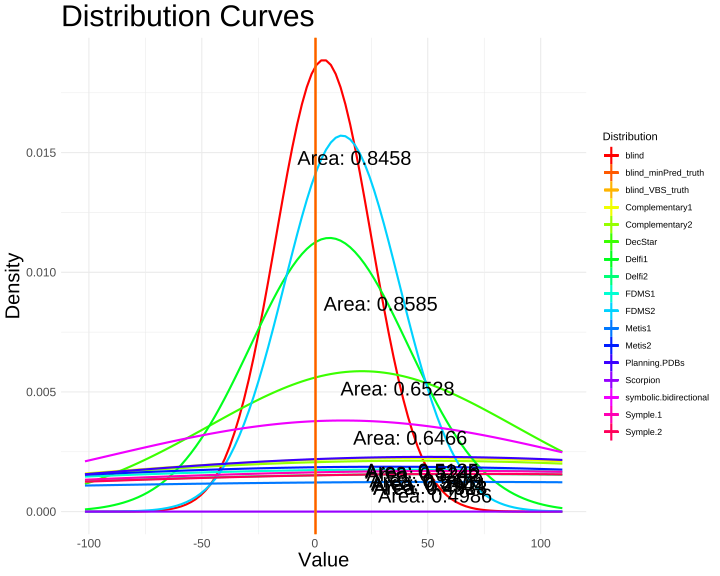
\includegraphics[width=.49\textwidth]{plots/Appendix/nurikabe_p03.pddl.pdf}
    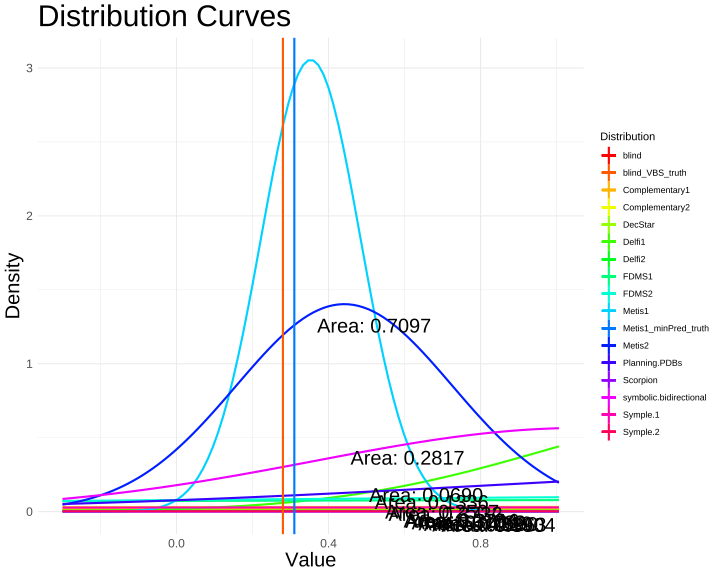
\includegraphics[width=.49\textwidth]{plots/Appendix/caldera_p03.pddl.pdf}
    \caption[Sub-portfolio Selection: Examples from IPC2018]{Sub-portfolio selection for two example instances from IPC2018 based on the optimal $p_{\cap}$ values}
    \label{fig:appendix_ipc2018}
\end{figure}
\begin{figure}
    \centering 
    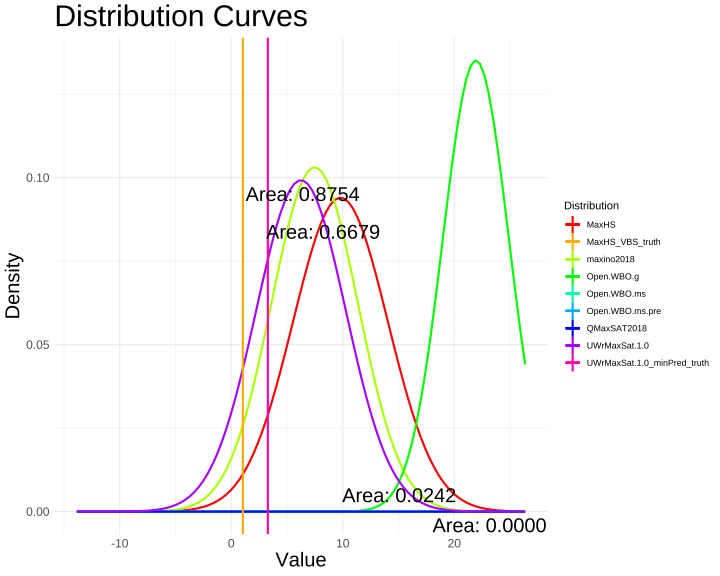
\includegraphics[width=.49\textwidth]{plots/Appendix/wolfram72_9.wcnf.pdf}
    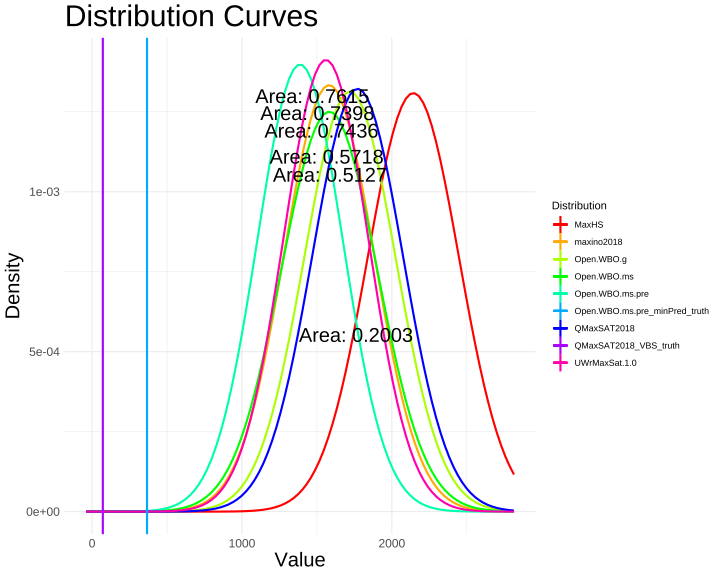
\includegraphics[width=.49\textwidth]{plots/Appendix/1bpi_2knt_gwcnft.wcnf.pdf}
    \caption[Sub-portfolio Selection: Examples from MAXSAT19-UCMS]{Sub-portfolio selection for two example instances from MAXSAT19-UCMS based on the optimal $p_{\cap}$ values}
    \label{fig:appendix_maxsat}
\end{figure}

% \begin{figure}[t]
% \centering
%     \centerline{\includegraphics[width=\linewidth]{plots/pcap_rj_sensitivity_x_theta_y_runtime_facet.pdf}}
%     \caption{Sensitivity of portfolio performance to $p_{\cap}$. This plot refers to RJ model - Regression Ranger model with Jackknife uncertainty estimation method. The plot illustrates the mean, Q1 (25th percentile), Q2 (50th percentile), and Q3 (75th percentile) runtime performance of each scenario for various values of $p_{\cap}$ as defined in Equation~\ref{eq:7}. Note the log scale for the normalized gap closed.}
%     \label{fig:sensitivity_pcap_ri}
% \end{figure} % appendix A
\input{uwyo_B} % appendix B

%% Uncomment the line below if you want abbreviations to be an appendix, at the end of the document
%\input{uwyo_C_abbr} % appendix C


% Generate the References section using BibTeX. Optionally you
% can code this by hand (argh!)
\bibliographystyle{ieeetr} % IEEE standard citation style
\addcontentsline{toc}{chapter}{\bibname} % make reference section show up in TOC

\begin{spacing}{1.0} % sets line spacing of references
% reads in the sample BibTex file supplied; change to your bib file name
\bibliography{sample}
\end{spacing}


%\begin{thesisauthorvita}
%This is where you put your vita if needed. Not usually used at UW.
%\end{thesisauthorvita}


%% all done!
\end{document}
